% !Mode:: "TeX:UTF-8"
% !TEX program = xelatex

\documentclass[bwprint]{report}

\title{大小模型协同的智能交通出行问答系统}
\stuname{程泽凯\quad 王晨羽\quad 金井直}
\stuclass{计算机2023-04版}
\supervisor{杜圣东}
\dateinput{\today}
\def\makeothertitle{}
\setlength{\cftsecnumwidth}{3.2em}
\setlength{\cftsubsecnumwidth}{4.4em}
\setlength{\cftsubsubsecnumwidth}{5.6em}

\begin{document}

\maketitle
\newpage

\pagestyle{plain}
\pagenumbering{Roman}
\begin{center}
    {\zihao{4}\bfseries 摘要}
\end{center}

本报告对应的课程设计题目为``大小模型协同的智能交通出行问答系统''。我们围绕成都市出行场景做了一个问答原型，重点不是把它做成正式交通服务平台，而是验证大模型、知识库、外部工具和前两次大作业模型能否在同一个流程里跑通。实现时，Dify 用来编排工作流，DeepSeek 小参数模型负责组织回答，并配合 LoRA/QLoRA 微调改善交通问答中的工具意识和回答边界。知识库采集了成都市交管局信息发布栏、交通法规和出行建议等资料，用于本地 RAG 检索；高德地图 API 和天气查询用于处理实时性较强的问题，知乎搜索只作为外部参考。项目还接入了 STAEformer 交通流预测模块和 YOLO 交通目标/交通标志识别模块。后端使用 FastAPI 统一封装接口，前端用三栏式页面展示回答、证据和可视化结果。测试时主要检查普通问答、RAG 证据、路线规划、天气提醒、交通流预测、图片识别和 Dify 调用链路是否能跑通。当前版本已经能够完成课程演示中的主要流程，但知识库规模、实时数据和交互细节仍然比较有限。

\vspace{0.5em}
\noindent{\heiti 关键词：}智能交通；Dify；检索增强生成；DeepSeek；高德地图；STAEformer；YOLO；交通问答

\newpage
\tableofcontents
\newpage
\pagestyle{plain}
\setcounter{page}{1}
\pagenumbering{arabic}

\section{团队成员分工}
系统实现与报告整理按以下模块分工：
\begin{itemize}
    \item 程泽凯：负责需求分析、交通知识库整理、RAG 检索方案和知乎搜索补充策略设计。
    \item 王晨羽：负责 FastAPI 后端、工具接口、高德 API、交通流预测与 YOLO 识别模块集成。
    \item 金井直：负责三栏前端界面、右侧证据可视化、Dify 工作流设计、一键启动脚本和报告排版。
\end{itemize}

\section{任务背景}
我们最开始考虑的是日常出行信息分散的问题。比如限行和施工公告一般要去交管网站或公众号查，路线规划要打开地图软件，天气影响又要看气象信息。用户如果只是想问一句``成都尾号限行怎么规定''、``雨天开车要注意什么''或``从天府广场到春熙路怎么走''，实际操作上往往要切换好几个入口。这类问题足够具体，也和智能交通课程内容比较贴近，因此适合作为本次课程设计的场景。

大语言模型确实方便用自然语言交互，但它并不适合单独回答交通政策和实时出行问题。调试时很容易看到类似情况：模型能把句子说得很完整，却可能把旧政策当作当前规则，或者直接估计路线耗时。为避免这种问题，本项目把本地 RAG、外部 API、交通流预测和图片识别都接入问答流程，让模型更多负责整理、解释和提示风险，而不是凭记忆决定事实。

大作业3还要求体现 Dify、DeepSeek 小参数模型、网络采集知识库、微调以及前两次大作业成果的集成。基于这些要求，我们把成都市交管局网站信息发布栏、交通法规和出行建议资料整理成本地 RAG 知识库，同时复用大作业1的 STAEformer 预测结果和大作业2的 YOLO 识别模型。项目目标比较明确：在课程设计范围内把问答、工具调用、证据展示和可视化结果串起来，而不是宣称已经完成一个可直接上线的交通服务系统。

\section{任务描述}
本项目的任务可以理解为两部分：一部分是面向成都市交通出行场景做一个能演示的问答系统，另一部分是把课程前两次大作业的模型结果接进来。具体实现中，我们使用 Dify 编排流程，采用 DeepSeek 开源 1--7B 级模型作为基座模型，并围绕问答、工具调用和证据展示完成以下内容：

\begin{enumerate}
    \item 网络采集成都市交管局网站信息发布栏内容，并结合交通法规、出行建议资料建立本地 RAG 出行知识库。
    \item 采用 DeepSeek 开源 1--7B 级模型作为基座模型，并进行面向交通问答场景的 LoRA/QLoRA 微调。
    \item 基于 Dify 开发框架构建可视化分支工作流，实现意图识别、工具编排和最终回答生成。
    \item 支持交管信息问答、天气问答、出行建议、出行路径规划等基础问答功能。
    \item 接入知乎搜索 API，在本地知识库之外提供外部补充信息，并明确标注其参考性质。
    \item 接入高德地图 API，实现路线规划结果获取和前端地图路线绘制。
    \item 集成大作业1 STAEformer 交通流预测能力，对成都演示地点进行未来一小时交通流趋势展示，并支持交通流预测问答。
    \item 集成大作业2 YOLO 交通目标/交通标志识别能力，支持用户上传图片并进行识别理解问答。
    \item 构建三栏式 HTML 问答界面，使回答、证据和可视化结果同步展示。
    \item 提供一键启动和停止脚本，方便课程演示和复现实验。
\end{enumerate}

在实现取舍上，我们没有把所有内容都交给聊天模型自由生成，而是把``回答文字''和``依据展示''分开。大模型负责把检索片段或工具结果整理成用户能读懂的回答；RAG 和外部工具提供事实依据；前端 panel 再把地图、知识片段、预测曲线或识别图展示出来。这样虽然实现上多了一层结构，但演示时更容易检查回答从哪里来。

\subsection{作业要求对应关系}
表\ref{tab:requirement-mapping} 列出了课程要求和本项目实现内容之间的对应关系。这里主要用于自查，避免报告里写了功能但系统中没有对应模块。

\begin{table}[H]
    \caption{大作业3要求与系统实现对应关系}
    \label{tab:requirement-mapping}
    \centering
    \small
    \begin{tabular}{p{0.30\textwidth}p{0.52\textwidth}}
        \toprule[1.5pt]
        作业要求 & 本系统实现 \\
        \midrule[1pt]
        基于 Dify 开发框架 & 构建中文节点分支式 Dify Workflow，通过后端代理调用工作流并复用本地工具接口。 \\
        DeepSeek 1--7B 基座模型 & 选用 \texttt{DeepSeek-R1-Distill-Qwen-7B}，并导入为本地 \texttt{travelqa} 模型。模型卡标注参数量为 7.62B，工程上按 7B 级蒸馏模型处理；若严格按不超过 7.00B 字面约束，可替换为同系列 1.5B 或 \texttt{deepseek-llm-7b-chat}。 \\
        网络采集成都市交管局信息发布栏 & 将成都市交管局信息发布栏、交通法规和出行建议资料清洗切分后写入本地 RAG 知识库。 \\
        构建本地 RAG 出行知识库 & 使用 Hybrid RAG 检索策略，结合语义检索、BM25 和证据片段展示。 \\
        对基座模型进行微调 & 在 AutoDL 环境中完成 LoRA/QLoRA 微调，并通过 SwanLab 记录训练过程。 \\
        交管信息、天气、建议、路径规划问答 & 通过意图识别分别调用 RAG、天气工具、高德路线规划和大模型回答生成。 \\
        集成交通流预测模型成果 & 复用大作业1 STAEformer，支持成都地点到 PEMS08 节点的演示映射和未来一小时预测。 \\
        集成交通目标识别模型成果 & 复用大作业2 YOLO 权重，支持图片上传、目标检测、标注图展示和识别理解问答。 \\
        完成作业报告 & 按课程设计模板生成本报告，并提供可复现实验步骤和测试结果。 \\
        \bottomrule[1.5pt]
    \end{tabular}
\end{table}

\section{总体技术方案}
\subsection{系统总体架构}
实际运行时，请求大致会经过前端、FastAPI 后端、意图识别和具体工具模块几个环节。我们把页面做成三栏，是为了把回答、依据和可视化结果同时摆出来；后端统一使用 FastAPI，是为了让本地页面和 Dify 工作流都能复用同一套接口。整体架构如图\ref{fig:architecture} 所示。

\begin{figure}[H]
    \centering
    \fbox{
    \begin{minipage}{0.92\textwidth}
    \small
    \begin{center}
    用户 $\rightarrow$ 三栏 Web 问答界面 $\rightarrow$ FastAPI 后端

    \vspace{0.4em}
    FastAPI 后端 $\rightarrow$ 意图识别 $\rightarrow$
    \{本地 RAG，知乎搜索，高德路线/天气，STAEformer，YOLO，Ollama 大模型\}

    \vspace{0.4em}
    FastAPI 后端 $\rightarrow$ panel 结构 $\rightarrow$
    \{地图路线，知识片段，预测曲线，YOLO 标注图\}

    \vspace{0.4em}
    Dify 模式：Web $\rightarrow$ FastAPI 代理 $\rightarrow$ Dify Workflow $\rightarrow$ TravelQA 工具接口
    \end{center}
    \end{minipage}}
    \caption{智能交通问答系统总体架构}
    \label{fig:architecture}
\end{figure}

本项目保留了本地模式和 Dify 模式两条链路。本地模式便于调试，前端直接请求 TravelQA 后端即可；Dify 模式用于展示可视化工作流，但调用时通过后端代理，避免把应用密钥放到浏览器里。右侧可视化面板没有交给 Dify 单独生成，而是继续由本地 TravelQA 后端返回 panel 数据。这样做的原因很简单：两种模式下页面表现更一致，也方便对比同一个问题在不同链路下的处理结果。

\subsection{关键技术栈}
本项目用到的主要技术栈见表\ref{tab:tech-stack}。

\begin{table}[H]
    \caption{系统关键技术栈}
    \label{tab:tech-stack}
    \centering
    \begin{tabular}{p{0.22\textwidth}p{0.30\textwidth}p{0.34\textwidth}}
        \toprule[1.5pt]
        层级 & 技术或工具 & 作用 \\
        \midrule[1pt]
        前端 & 原生 HTML/CSS/JavaScript & 三栏问答界面、地图、图表和图片展示 \\
        后端 & FastAPI、Uvicorn & 问答接口、工具接口、静态资源托管 \\
        大模型 & DeepSeek-R1-Distill-Qwen-7B、Ollama 本地模型 travelqa & 作为 1--7B 级基座和微调后推理模型，根据证据和工具结果生成自然语言回答 \\
        检索 & BGE-M3、BM25、Reranker & 面向成都市交管局信息发布栏和交通法规资料的本地知识库 Hybrid RAG \\
        外部搜索 & 知乎搜索 API & 本地知识库之外的补充参考 \\
        地图服务 & 高德 Web 服务 API、JS API & 路线规划、地理编码和前端地图绘制 \\
        预测模型 & STAEformer & 未来一小时交通流趋势预测 \\
        视觉模型 & YOLO、TT100K & 交通目标/交通标志识别和标注图生成 \\
        工作流 & Dify 1.14.2 & 可视化意图分支和工具编排 \\
        部署脚本 & PowerShell、Docker Compose & 一键启动、停止与健康检查 \\
        \bottomrule[1.5pt]
    \end{tabular}
\end{table}

\subsection{系统功能介绍}
功能上，页面把普通交通问答、外部工具、小模型预测和图片识别放在一起。用户输入自然语言问题后，后端根据意图选择不同链路；中间区域展示回答，右侧区域展示证据或图形结果。这样设计主要是为了课堂演示时不用在多个窗口之间来回切换。

\begin{table}[H]
    \caption{系统主要功能说明}
    \label{tab:system-functions}
    \centering
    \small
    \begin{tabular}{p{0.20\textwidth}p{0.30\textwidth}p{0.34\textwidth}}
        \toprule[1.5pt]
        功能类别 & 典型问题或输入 & 系统处理方式 \\
        \midrule[1pt]
        交管信息问答 & 成都尾号限行、交通管制、违法处罚等 & 优先检索本地 RAG 知识库，必要时补充知乎搜索，并提示以官方发布为准 \\
        天气问答 & 成都今天是否下雨、雨天出行是否安全 & 调用天气工具获取天气信息，再由大模型生成出行提示 \\
        出行建议 & 下雨天开车要注意什么、事故后如何处理 & 检索法规和安全驾驶建议，结合大模型生成结构化建议 \\
        出行路径规划 & 从天府广场到春熙路怎么走 & 抽取起终点，调用高德路线规划 API，右侧展示地图路线和步骤 \\
        交通流预测问答 & 春熙路未来一小时交通流如何 & 将成都地点名映射到 PEMS08 节点，调用 STAEformer 预测并绘制折线图 \\
        交通目标识别理解 & 上传交通标志图片 & 调用 YOLO 识别交通标志，生成标注图、类别、置信度和解释回答 \\
        Dify 工作流模式 & 切换到 Dify 后继续提问 & 通过 Dify 分支工作流完成意图识别和工具编排，前端仍展示本地证据面板 \\
        \bottomrule[1.5pt]
    \end{tabular}
\end{table}

\section{核心模块设计}
\subsection{意图识别模块}
意图识别是后端进入各类工具前的第一步。当前版本没有把这一步做得很复杂，而是先用规则关键词把用户问题分到几个处理路径中。支持的主要意图包括：
\begin{itemize}
    \item \texttt{traffic-info}：交通政策、限行、违法处罚、管制等信息。
    \item \texttt{travel-advice}：雨天驾驶、事故处理、出行建议等。
    \item \texttt{weather}：天气、气温、降雨、能见度等。
    \item \texttt{route}：从某地到某地的路线规划和导航。
    \item \texttt{forecast}：交通流、车流、拥堵趋势和未来预测。
    \item \texttt{detection}：交通标志识别、YOLO、图片检测能力。
\end{itemize}

这里采用规则方式，主要是为了演示稳定。课程验收时如果同一句问题每次都被分到不同分支，后面的地图、预测或 RAG 结果就很难复查。对于路线规划，后端还会调用 \texttt{extract\_route\_od} 从句子中抽取起点和终点。例如用户输入``我从天府广场到春熙路怎么走''时，系统会解析出起点为天府广场、终点为春熙路，然后进入路线规划工具。本地 FastAPI 原型目前主要依赖关键词规则；Dify 工作流中的``意图识别''节点后续可以换成 LLM 分类节点，只要求模型输出 \texttt{route}、\texttt{forecast}、\texttt{weather}、\texttt{detection}、\texttt{traffic-info} 或 \texttt{travel-advice} 六类标签即可。

本地路由核心代码如下。规则顺序按工具信号的明确程度排列：路线、预测、识别、天气先匹配，限行和违章等交通政策关键词再进入 RAG，最后兜底到 \texttt{traffic-info}。调试时发现，``从 A 到 B 堵不堵''、``实时路况''、``避堵路线''这类问法表面上像交通咨询，但实际更接近路线规划。如果不额外处理，很容易被分到普通 RAG，所以后面补充了这些路线规划信号。

\begin{lstlisting}[language=Python]
_RULES = [
    (Intent.ROUTE, ["怎么去", "怎么走", "路线", "路径", "导航",
                    "从.*到.*堵", "实时路况", "避堵路线"]),
    (Intent.FORECAST, ["交通流", "预测", "未来.*车流", "mae", "staeformer"]),
    (Intent.DETECTION, ["识别", "检测", "标志", "yolo", "tt100k"]),
    (Intent.WEATHER, ["天气", "气温", "降水", "会不会下雨"]),
    (Intent.TRAFFIC_INFO, ["限行", "尾号", "违章", "管制", "施工"]),
    (Intent.TRAVEL_ADVICE, ["建议", "注意", "事故", "快处", "追尾"]),
]

def classify(query: str) -> Intent:
    q = query.lower()
    for intent, patterns in _RULES:
        for pat in patterns:
            if re.search(pat, q):
                return intent
    return Intent.TRAFFIC_INFO
\end{lstlisting}

\subsection{本地 RAG 模块}
RAG 模块处理的是``回答有没有依据''这个问题。项目把成都市交管局网站信息发布栏、道路交通安全相关法规、常见驾驶安全建议和项目整理的问答材料放入本地知识库。遇到限行、处罚、施工公告或驾驶建议这类问题时，后端先检索知识片段，再把片段交给模型组织回答。对政策公告类内容，chunk 元数据里保留标题、来源信息、发布时间或抓取时间，右侧证据面板才能把出处显示出来。

检索没有只用向量相似度，而是采用 Hybrid Search，把语义向量检索和 BM25 关键词检索结合起来。原因是交通问题里路名、区域名、日期和政策关键词很重要，语义上相近并不代表事实上匹配。例如两个施工公告都和``交通管制''有关，但道路和时间不同，答案就不能混用。

本地 RAG 流程如下：
\begin{enumerate}
    \item 网络采集成都市交管局信息发布栏，并导入交通法规、公告网页、出行建议或 PDF。
    \item 文档清洗与格式统一，将网页正文、标题、发布时间、来源信息转换为结构化文本。
    \item 文本切分为 chunk，保留标题、发布时间、来源和正文片段。
    \item 使用 BGE-M3 或离线哈希向量生成文本向量。
    \item 构建 BM25 关键词索引。
    \item 查询时同时执行向量检索和关键词检索。
    \item 使用 RRF 或重排序模型融合结果。
    \item 将命中片段作为 evidence 输入大模型。
\end{enumerate}

在实现上，RAG 不是简单地把文本搜出来。前面要做网页或 PDF 清洗、切分和索引构建；查询时还要融合向量召回和关键词召回；最后还要把命中的片段整理成前端能展示的证据。具体流程见表\ref{tab:rag-flow}。

\begin{table}[H]
    \caption{本地 RAG 全流程}
    \label{tab:rag-flow}
    \centering
    \small
    \begin{tabular}{p{0.18\textwidth}p{0.26\textwidth}p{0.40\textwidth}}
        \toprule[1.5pt]
        阶段 & 输入/输出 & 说明 \\
        \midrule[1pt]
        数据采集 & 成都市交管局信息发布栏、法规网页、PDF、出行建议资料 & 采集时保留来源信息、标题、发布时间或抓取时间，便于后续追溯 \\
        文档清洗 & 原始 HTML/PDF $\rightarrow$ 纯文本 & 去除导航栏、页脚和重复文本，统一编码和段落结构 \\
        结构化切分 & 文档 $\rightarrow$ chunks & 按语义段落切分，并保留 category、district、road、valid\_time 等元数据 \\
        索引构建 & chunks $\rightarrow$ 向量索引与 BM25 索引 & 语义检索负责相近表达匹配，BM25 负责政策关键词、路名和时间等精确匹配 \\
        查询理解 & 用户问题 $\rightarrow$ 意图和检索 query & 识别交通政策、出行建议、天气、路线、预测或识别等意图 \\
        混合检索 & query $\rightarrow$ 候选片段 & 同时执行向量检索和关键词检索，避免单一路径漏召回 \\
        结果融合 & 候选片段 $\rightarrow$ Top-K 证据 & 使用融合排序或重排序策略筛选最相关片段 \\
        外部补充 & query $\rightarrow$ 知乎搜索片段 & 即使本地知识库命中，也补充搜索一次，但在回答中明确其仅供参考 \\
        回答生成 & evidence + query $\rightarrow$ answer & 大模型基于本地证据优先生成回答，不把外部补充当作官方结论 \\
        证据展示 & chunks $\rightarrow$ panel & 前端右侧展示标题、摘要、来源和时间信息，方便用户核验 \\
        \bottomrule[1.5pt]
    \end{tabular}
\end{table}

前端右侧会展示本轮命中的知识片段，包括标题、正文摘要、来源信息、发布时间或抓取时间。这样做不是为了把页面做复杂，而是为了让用户看到回答后能顺手检查依据是否可信。

当前知识库与检索配置见表\ref{tab:rag-stats}。索引文件 \texttt{data/kb/index.json} 中为每个 chunk 保留 \texttt{id}、\texttt{text}、\texttt{title}、\texttt{url}、\texttt{fetched\_at}、\texttt{published\_at}、\texttt{category}、\texttt{district}、\texttt{road} 和 \texttt{valid\_time} 等元数据。因为这些字段还在，前端才能展示出处，而不是只展示一段模型生成的文字。

\begin{table}[H]
    \caption{RAG 知识库与检索配置}
    \label{tab:rag-stats}
    \centering
    \small
    \begin{tabular}{p{0.30\textwidth}p{0.48\textwidth}}
        \toprule[1.5pt]
        项目 & 当前配置或结果 \\
        \midrule[1pt]
        原始来源文档 & 18 篇，包括成都市交管局公告索引、交通法规、开放交通数据和出行建议资料 \\
        知识片段数 & 287 个 chunk \\
        向量模型 & \texttt{models/rag/bge-m3} \\
        Embedding provider & \texttt{sentence\_transformers} \\
        检索模式 & \texttt{hybrid}，向量检索 + BM25，RRF 融合 \\
        最终 Top-K & \texttt{top\_k=4}，重排序后送入大模型 \\
        重排序模型 & \texttt{models/rag/bge-reranker-v2-m3} \\
        过滤阈值 & \texttt{min\_score=0.05} \\
        \bottomrule[1.5pt]
    \end{tabular}
\end{table}

Hybrid Search 的核心实现如下。代码中先分别得到向量召回和 BM25 召回，再用 Reciprocal Rank Fusion 合并两路排名，最后把候选结果交给 Reranker 做二次排序。

\begin{lstlisting}[language=Python]
def hybrid_search(self, query, query_vec, top_k=4,
                  vector_top_k=20, bm25_top_k=20, rrf_k=60):
    vec_hits = self.vector_search(query_vec, top_k=vector_top_k)
    bm25_hits = self.bm25_search(query, top_k=bm25_top_k)
    fused = {}
    for rank, (idx, _) in enumerate(vec_hits):
        fused[idx] = fused.get(idx, 0.0) + 1.0 / (rrf_k + rank + 1)
    for rank, (idx, _) in enumerate(bm25_hits):
        fused[idx] = fused.get(idx, 0.0) + 1.0 / (rrf_k + rank + 1)
    ranked = sorted(fused.items(), key=lambda x: x[1], reverse=True)
    return [self._to_hit(sc, self._meta[idx]) for idx, sc in ranked[:top_k]]
\end{lstlisting}

\subsection{基座模型选择与模型介绍}
大模型基座选用 \texttt{DeepSeek-R1-Distill-Qwen-7B}，模型来自 DeepSeek-R1 系列蒸馏模型，可从 ModelScope 开源模型页面获取。选它主要是出于课程设计的工程条件考虑：完整大模型不适合在本地或普通云端环境里反复调试，而 7B 级蒸馏模型在部署和微调成本上更容易接受，中文表达能力也基本够用。需要注意的是，模型卡标注参数量为 7.62B，工程上按 7B 级蒸馏模型使用。

\begin{table}[H]
    \caption{DeepSeek-R1-Distill-Qwen-7B 模型卡片}
    \label{tab:deepseek-model-card}
    \centering
    \begin{tabular}{p{0.30\textwidth}p{0.48\textwidth}}
        \toprule[1.5pt]
        项目 & 内容 \\
        \midrule[1pt]
        模型名称 & DeepSeek-R1-Distill-Qwen-7B \\
        模型来源 & ModelScope 开源模型仓库 \\
        参数量 & 7.62B \\
        基础模型系列 & Qwen 系列蒸馏基座 \\
        权重格式 & Safetensors \\
        深度学习框架 & PyTorch \\
        张量类型 & BF16 \\
        开源协议 & MIT \\
        模型大小 & 15.24 GB \\
        更新时间 & 2025 年 2 月 25 日 \\
        \bottomrule[1.5pt]
    \end{tabular}
\end{table}

与完整 DeepSeek-R1 相比，7B 级蒸馏模型更适合本次课程设计。它的体积处在个人工作站或云端单卡环境可以处理的范围内，便于 QLoRA 训练、Ollama 本地推理和课堂演示。这里还做了一个边界划分：模型不直接计算路线距离、天气或交通流，而是在 RAG、地图、天气、预测和识别工具给出结果后，负责把这些结果整理成回答。

公开模型介绍中给出的蒸馏模型评测结果如表\ref{tab:deepseek-benchmark} 所示。这里引用这些指标不是为了把数学或代码评测结果直接迁移到交通问答上，而是说明该模型有一定的信息整理和步骤化表达能力。实际项目里，路线步骤解释、预测趋势说明和法规依据整理都需要这种能力。

\begin{table}[H]
    \caption{DeepSeek-R1-Distill-Qwen-7B 公开评测指标}
    \label{tab:deepseek-benchmark}
    \centering
    \begin{tabular}{p{0.36\textwidth}p{0.28\textwidth}}
        \toprule[1.5pt]
        评测项目 & 指标值 \\
        \midrule[1pt]
        AIME 2024 pass@1 & 55.5 \\
        AIME 2024 cons@64 & 83.3 \\
        MATH-500 pass@1 & 92.8 \\
        GPQA Diamond pass@1 & 49.1 \\
        LiveCodeBench pass@1 & 37.6 \\
        CodeForces rating & 1189 \\
        \bottomrule[1.5pt]
    \end{tabular}
\end{table}

官方使用建议中提到，推理时温度可设置在 0.5 至 0.7 区间，并建议减少复杂系统提示词对模型行为的干扰。本项目实际采用``先拿证据和工具结果，再让模型组织语言''的方式：本地 RAG、知乎搜索、高德 API、STAEformer 和 YOLO 先生成结构化 evidence，再由本地 \texttt{travelqa} 模型输出最终回答。为了避免前端出现长篇推理过程，Ollama provider 中固定使用 \texttt{think=false}，提示词也只要求输出结论、依据和注意事项。

\subsection{大模型微调模块}
除了 RAG 与工具调用，项目还完成了面向交通问答场景的大模型微调。微调基座模型为 \texttt{DeepSeek-R1-Distill-Qwen-7B}，训练方式采用 LoRA/QLoRA 思路，也就是冻结大部分基座参数，只训练低秩适配器参数。这里的目标不是让模型背交通公告。政策类内容变化很快，背下来反而容易过期；微调更希望让模型学会工具调用意识、RAG 证据引用方式、交通问答格式，以及不确定时不要乱答。

训练数据由离线脚本生成，统一保存为 Alpaca 风格 JSONL。每条样本至少包含 \texttt{instruction}、\texttt{input} 和 \texttt{output} 三个字段，并附加 \texttt{category}、\texttt{source} 和 \texttt{group\_id} 用于检查来源。划分训练集和验证集时，脚本用 \texttt{group\_id} 做隔离，避免同一事实或同一工具场景的不同说法同时出现在两边。

\begin{lstlisting}
{
  "instruction": "成都公共数据开放平台是否收录某交通资源？怎样获取？",
  "input": "",
  "output": "开放目录元数据显示，该资源由对应部门提供。目录元数据不等于数据正文。",
  "category": "open_catalog",
  "source": "chengdu-open-catalog",
  "group_id": "open_catalog:..."
}
\end{lstlisting}

微调数据集统计见表\ref{tab:sft-stats}。数据不只包含少量手写问答，还覆盖了公交、轨道、停车、开放目录、路线工具、天气工具、预测、识别、拒答和工具不可用等场景。这样做是为了让模型在遇到实时问题或缺少工具结果时，不要直接给出看似确定的答案。

\begin{table}[H]
    \caption{LoRA/QLoRA 微调数据集统计}
    \label{tab:sft-stats}
    \centering
    \small
    \begin{tabular}{p{0.32\textwidth}p{0.46\textwidth}}
        \toprule[1.5pt]
        项目 & 数值或说明 \\
        \midrule[1pt]
        样本总数 & 1228 条 SFT 样本 \\
        训练集 / 验证集 & 1104 / 124 \\
        数据划分随机种子 & 20260601 \\
        group 泄漏检查 & 0，训练集和验证集无同组语义泄漏 \\
        主要类别 & bus 320、metro 252、parking 198、open\_catalog 160、refusal 80、tool\_call 40、toll\_station 38 \\
        高阶集成类别 & forecast 20、detection 20、route 8、weather 8、tool\_unavailable 8 \\
        数据源审计 & 新都公交 87 行；成都市开放目录原始 7408 行，筛选 160 行进入 SFT \\
        \bottomrule[1.5pt]
    \end{tabular}
\end{table}

本次训练在 AutoDL 容器环境中完成。训练脚本加载 DeepSeek 基座模型和交通问答训练集，按 LoRA/QLoRA 参数训练 2 个 epoch，训练结束后保存适配器。

训练过程使用 SwanLab 进行实验跟踪。SwanLab 记录的关键信息如下：
\begin{itemize}
    \item 实验名称：DeepSeek 交通问答 LoRA 微调实验。
    \item 运行标识：SwanLab 自动生成的本次实验记录编号。
    \item 开始时间：2026 年 6 月 2 日 10:21:50
    \item 运行时间：5 分钟 19 秒
    \item SwanLab 版本：0.7.19
    \item 输出结果：训练日志、评估指标和 LoRA 适配器。
\end{itemize}

训练环境为 Ubuntu 22.04.5 LTS，Python 版本为 3.12.3。训练共进行 2 个 epoch，总步数为 138 步。日志显示，loss 从初始阶段的 3.6966 下降到第 1 个 epoch 附近约 1.0 左右，说明模型较快适应了训练数据中的输出格式。训练最终指标见表\ref{tab:lora-training-metrics}。

\begin{table}[H]
    \caption{DeepSeek-R1-Distill-Qwen-7B LoRA 微调指标}
    \label{tab:lora-training-metrics}
    \centering
    \begin{tabular}{p{0.30\textwidth}p{0.45\textwidth}}
        \toprule[1.5pt]
        指标 & 数值 \\
        \midrule[1pt]
        训练轮数 & 2 epoch \\
        总训练步数 & 138 steps \\
        训练运行时间 & 313.7957 s \\
        train\_samples\_per\_second & 7.036 \\
        train\_steps\_per\_second & 0.44 \\
        train\_loss & 1.1065 \\
        第 1 轮 eval\_loss & 0.9677 \\
        第 2 轮 eval\_loss & 0.9193 \\
        eval\_samples\_per\_second & 16.055 \\
        eval\_steps\_per\_second & 16.055 \\
        \bottomrule[1.5pt]
    \end{tabular}
\end{table}

训练曲线中，loss 在前半个 epoch 内下降比较明显：0.07 epoch 时 loss 为 3.6966，0.36 epoch 时降至 1.1901，0.72 epoch 时进一步降至 0.9854。第 2 个 epoch 中，loss 多数维持在 0.6 至 0.9 区间，最终训练平均损失为 1.1065。验证损失从第 1 轮的 0.9677 降至第 2 轮的 0.9193，说明这次微调在验证集上没有明显发散。梯度范数整体处于约 0.79 至 1.52 之间。

微调后的 LoRA 适配器可以与基座模型合并，也可以在推理时单独加载。本地项目最终通过 Ollama 导入为 \texttt{travelqa} 模型，并由 \texttt{config.yaml} 中的 \texttt{ollama\_native} provider 调用。这样处理后，回答风格更接近交通问答场景，尤其是工具结果解释和 RAG 证据组织这一类内容。

只看训练 loss 不足以说明微调真的有用，所以项目还提供 \texttt{finetune/ab\_eval.py}。脚本构建 100 条 holdout 问题，让未微调基座模型和加载 LoRA 后模型分别生成回答，再导出 CSV 与 HTML 页面供人工评分。当前已生成的 \texttt{ab\_eval\_v4/ab\_results.json} 中保存了两组输出。表\ref{tab:lora-ab-examples} 给出部分样例。对比时可以看到，基座模型容易直接猜测实时路线、天气或公告细节；微调后模型更倾向于先要求调用工具、引用公告来源，或者在缺少图片时拒绝判断。

\begin{table}[H]
    \caption{微调前后代表性输出对比}
    \label{tab:lora-ab-examples}
    \centering
    \scriptsize
    \begin{tabular}{p{0.24\textwidth}p{0.30\textwidth}p{0.30\textwidth}}
        \toprule[1.5pt]
        问题 & 未微调基座模型倾向 & 加载 LoRA 后倾向 \\
        \midrule[1pt]
        现在从成都东站开车到春熙路大约需要多久？ & 直接给出约 20--30 分钟，并展开路线猜测。 & 要求先调用 \texttt{route\_plan}，收到工具结果后再回答，不编造距离或耗时。 \\
        成都今天下午会下雨吗？出门需要带伞吗？ & 编造温度、风向和降雨概率。 & 说明不能凭空判断未来天气，需要查询实时天气或气象台预报。 \\
        请介绍最近的成都交管施工绕行通知，并给出可核验来源。 & 输出占位式的绕行路线、实施时间和政策范围。 & 要求先检索公告或调用工具，不能编造道路、限行或收费信息。 \\
        没有上传图片时，能判断前方一定有禁止停车标志吗？ & 能给出拒答，但仍带有较长推理过程。 & 明确说明缺少图片无法确认，应补充图片并结合实时路况核验。 \\
        \bottomrule[1.5pt]
    \end{tabular}
\end{table}

在样例对比之外，项目使用 \texttt{eval/score\_ab\_eval.py} 对 100 条 holdout 输出进行规则化评分。评分规则只检查这次微调重点关注的行为：是否要求调用工具、查询实时来源或拒绝不当请求，是否出现疑似编造的实时数值，是否泄漏 \texttt{<think>} 推理过程。这个评分比较机械，不能代替人工语义判断，但它可以重复运行，也便于检查微调前后回答边界的变化。结果见表\ref{tab:lora-ab-score}。

\begin{table}[H]
    \caption{微调前后 100 条 holdout 规则化评分}
    \label{tab:lora-ab-score}
    \centering
    \small
    \begin{tabular}{p{0.30\textwidth}p{0.22\textwidth}p{0.22\textwidth}}
        \toprule[1.5pt]
        指标 & 未微调基座 & 加载 LoRA 后 \\
        \midrule[1pt]
        样本数 & 100 & 100 \\
        合规回答数 & 22 & 90 \\
        合规率 & 22.0\% & 90.0\% \\
        疑似编造数值条数 & 20 & 0 \\
        疑似编造率 & 20.0\% & 0.0\% \\
        \texttt{<think>} 泄漏条数 & 60 & 0 \\
        \bottomrule[1.5pt]
    \end{tabular}
\end{table}

按类别看，LoRA 在路线工具、天气工具、停车实时余位、隐私拒答、工具不可用、公告依据和图片识别等场景变化比较明显。例如路线工具类 12 条中，微调后 12 条都要求先调用路线工具或避免编造耗时；隐私拒答类 10 条中，微调后 10 条都明确拒绝提供个人车主、轨迹或联系方式信息。少数开放目录和预测类问题仍有不足，主要原因是规则化评分要求回答中显式出现工具或核验词，而部分正确回答使用了更自然的说法，未必被规则命中。

规则化评分不能判断整体回答是否自然，因此项目又从 100 条 holdout 输出中抽取 20 条小样本，覆盖路线、天气、停车、隐私、工具不可用、公告依据、公交地铁、预测和图片识别等类别，按 helpfulness、依据/工具意识、边界控制三个维度进行人工盲评复核。评分文件为 \texttt{eval/ab\_blind\_review\_20.json}，摘要脚本为 \texttt{eval/summarize\_ab\_blind\_review.py}。结果见表\ref{tab:lora-manual-review}。

\begin{table}[H]
    \caption{微调前后 20 条人工盲评复核}
    \label{tab:lora-manual-review}
    \centering
    \small
    \begin{tabular}{p{0.30\textwidth}p{0.22\textwidth}p{0.22\textwidth}}
        \toprule[1.5pt]
        指标 & 未微调基座 & 加载 LoRA 后 \\
        \midrule[1pt]
        平均质量分（0--5） & 1.65 & 4.25 \\
        胜出样本数 & 1 & 17 \\
        平局样本数 & \multicolumn{2}{c}{2} \\
        主要问题 & 编造实时数值、泄漏推理 & 个别回答过短或工具名不够精确 \\
        \bottomrule[1.5pt]
    \end{tabular}
\end{table}

人工复核结果与规则化评分方向基本一致：微调后模型在不编造实时结果、拒绝隐私请求和要求调用工具方面更稳一些。不过评审中也保留了两个边界问题：一是个别停车问题中工具建议不够贴切，二是交通标志置信度解释时回答过于保守，没有把置信度含义说明清楚。这些样例已保存在评审 JSON 中，后续可以继续补充到数据集里。

\subsection{知乎搜索补充模块}
知乎搜索模块使用知乎开放 API 进行站内搜索，搜索结果包括标题、摘要、来源地址、作者、赞同数、评论数和更新时间。加入这个模块时，我们把它定位为补充参考，而不是官方依据。原因也比较直接：知乎内容更新快、说法多，但并不适合直接作为交通政策结论。

因此，本地知识库的优先级始终高于知乎搜索。即使本地知识库已有命中，后端也会额外搜索一次知乎，但回答中会明确标注：
\begin{itemize}
    \item 知乎搜索内容仅供参考。
    \item 不代表官方结论。
    \item 对时效性政策、处罚和临时管制，以官方发布为准。
\end{itemize}

对于``成都尾号限行怎么规定''一类强时效问题，后端会检查知乎结果时间。较旧结果只作为历史参考，不直接当成当前规则输出，避免把过期回答误认为现行政策。

\subsection{路线规划与地图模块}
识别到路线意图后，后端调用高德 Web 服务 API 完成 POI 解析、地理编码和驾车路径规划。路线结果包括起点、终点、距离、预计耗时、导航步骤和 polyline 坐标串。

前端只获取地图绘制所需的安全配置，并在右侧面板中使用高德地图路线规划能力绘制导航线路。实际调试时考虑到 Key 可能没有配置，页面没有直接依赖地图组件成功加载；如果前端地图配置缺失，就使用后端返回的路线坐标生成降级简图，并继续展示路线摘要。

路线规划模块的分工比较明确：路径距离、耗时和路线步骤由高德 API 提供，大模型只负责把结果整理成回答。这样做主要是为了避免模型凭空估计路线和时间。

\subsection{交通流预测模块}
交通流预测模块复用大作业1中的 STAEformer 结果。这里有一个必须说明的限制：当前项目面向成都演示场景，但底层预测数据来自 PEMS08，并不是成都真实检测器数据。因此系统采用固定的``成都地点名到 PEMS08 node\_id''演示映射。用户可以用熟悉的成都地名提问，后端再映射到底层节点完成预测。

例如：
\begin{itemize}
    \item 春熙路映射到 node\_id=12。
    \item 成都东站映射到 node\_id=24。
    \item 熊猫基地映射到 node\_id=108。
\end{itemize}

回答文本和右侧面板都会说明该映射是演示用模拟映射，不是真实成都传感器数据。右侧面板绘制未来 60 分钟交通流折线图，并展示 rising、falling 或 stable 等趋势信息。

\subsection{交通标志识别模块}
交通标志识别模块复用大作业2的 YOLO 交通标志检测模型。用户上传图片后，后端先接收并临时保存图片，再调用检测模型推理，最后生成带框标注图供右侧面板展示。这里没有让大模型直接根据图片描述猜测标志，而是先看 YOLO 是否检测到已训练类别。

检测结果包括：
\begin{itemize}
    \item 交通标志类别。
    \item 置信度。
    \item 边界框坐标。
    \item 标注图访问地址。
\end{itemize}

前端右侧显示标注图和检测列表。若未检测到已训练类别，系统会返回``未识别到已训练交通标志类别''，而不是强行输出不确定猜测。

\subsection{Dify 工作流模块}
Dify 工作流主要用于可视化编排和课程验收展示。工作流已导出为平台可导入的格式，方便在新环境中复现。当前工作流共有 16 个节点、19 条边，节点均使用中文名，包括开始、意图识别、按意图分流、路线规划接口、交通流预测接口、本地 RAG 与知乎补充、合并分支回答和最终回复等。Dify 运行在容器中，通过容器到宿主机的内部访问通道调用 TravelQA 后端工具能力。

工作流按问题类型分支处理。路线问题调用路线接口，预测问题调用预测接口，天气问题调用天气接口，识别问题调用检测摘要接口，其余普通交通问题进入本地 RAG 与知乎补充分支。

Dify 节点职责见表\ref{tab:dify-nodes}。这些节点把用户输入、意图分类、分支调用、结果格式化和最终回复串到一起。相比只在代码里写路由，Dify 的好处是验收时能直观看到请求走到了哪条分支。

\begin{table}[H]
    \caption{Dify 工作流节点职责说明}
    \label{tab:dify-nodes}
    \centering
    \small
    \begin{tabular}{p{0.22\textwidth}p{0.20\textwidth}p{0.42\textwidth}}
        \toprule[1.5pt]
        节点名称 & 节点类型 & 作用说明 \\
        \midrule[1pt]
        开始 & Start & 接收用户问题、会话信息和前端传入的上下文变量 \\
        意图识别 & LLM/分类 & 将自然语言问题分类为路线、预测、天气、识别或 RAG 问答 \\
        按意图分流 & 条件分支 & 根据意图把请求路由到对应工具节点 \\
        路线规划接口 & HTTP & 调用 TravelQA 后端路线工具，返回起终点、距离、耗时和路径步骤 \\
        整理路线回答 & Code/LLM & 将路线工具 JSON 转换成可读回答和简要摘要 \\
        预测参数映射 & Code & 把成都地点名映射为 PEMS08 node\_id 和演示路段名称 \\
        交通流预测接口 & HTTP & 调用 STAEformer 预测接口，获得未来 60 分钟交通流序列 \\
        整理预测回答 & Code/LLM & 解释预测趋势，并说明成都地点名为演示映射 \\
        天气接口 & HTTP & 调用天气工具获取城市天气、温度和降雨等信息 \\
        整理天气建议 & Code/LLM & 将天气结果转换为出行建议 \\
        标志识别能力接口 & HTTP & 获取 YOLO/TT100K 支持类别和训练指标摘要 \\
        整理识别说明 & Code/LLM & 回答系统能识别哪些交通标志及其含义 \\
        本地 RAG 与知乎补充 & HTTP & 调用本地 RAG 与知乎补充链路，返回证据片段和参考来源 \\
        整理 RAG 回答 & Code/LLM & 按本地知识库优先原则组织政策、法规或出行建议回答 \\
        合并分支回答 & Variable/Code & 统一不同分支的回答字段，保证最终节点输入一致 \\
        最终回复 & Answer & 向用户返回本轮最终回答 \\
        \bottomrule[1.5pt]
    \end{tabular}
\end{table}

Dify 的分支执行流程见表\ref{tab:dify-flows}。每条分支先拿到结构化工具结果，再交给整理节点转成自然语言，最后由统一回复节点输出。前端在 Dify 模式下仍复用本地后端生成的证据面板，所以右侧地图、RAG 片段、预测曲线和识别结果与本地模式保持一致。这个设计在调试时比较省事，因为不用维护两套不同的可视化逻辑。

\begin{table}[H]
    \caption{Dify 工作流分支流程说明}
    \label{tab:dify-flows}
    \centering
    \small
    \begin{tabular}{p{0.18\textwidth}p{0.32\textwidth}p{0.36\textwidth}}
        \toprule[1.5pt]
        流程类型 & 节点流转 & 输出内容 \\
        \midrule[1pt]
        路线规划流程 & 开始、意图识别、按意图分流、路线规划接口、整理路线回答、合并分支回答、最终回复 & 起终点、距离、预计耗时、主要导航步骤和右侧地图路线证据 \\
        交通流预测流程 & 开始、意图识别、按意图分流、预测参数映射、交通流预测接口、整理预测回答、合并分支回答、最终回复 & 成都地点名、演示映射节点、未来 60 分钟预测序列、趋势判断和折线图 \\
        天气出行流程 & 开始、意图识别、按意图分流、天气接口、整理天气建议、合并分支回答、最终回复 & 天气状态、温度、降雨信息和面向出行的安全建议 \\
        标志识别流程 & 开始、意图识别、按意图分流、标志识别能力接口、整理识别说明、合并分支回答、最终回复 & 可识别交通标志类别、检测能力说明和图片识别入口提示 \\
        RAG 问答流程 & 开始、意图识别、普通交通问答分支、本地 RAG 与知乎补充、整理 RAG 回答、合并分支回答、最终回复 & 本地知识库依据、知乎补充参考、来源优先级说明和政策时效提醒 \\
        统一回复流程 & 各工具分支、合并分支回答、最终回复 & 将不同分支的结果整理为统一回答字段，保证前端显示稳定 \\
        \bottomrule[1.5pt]
    \end{tabular}
\end{table}

图\ref{fig:dify-workflow-full} 展示了 Dify 工作流的全景结构。工作流从开始节点进入意图识别，再由条件分支路由到路线、预测、天气、识别和 RAG 等链路，最后汇总到统一回复节点。

\begin{figure}[H]
    \centering
    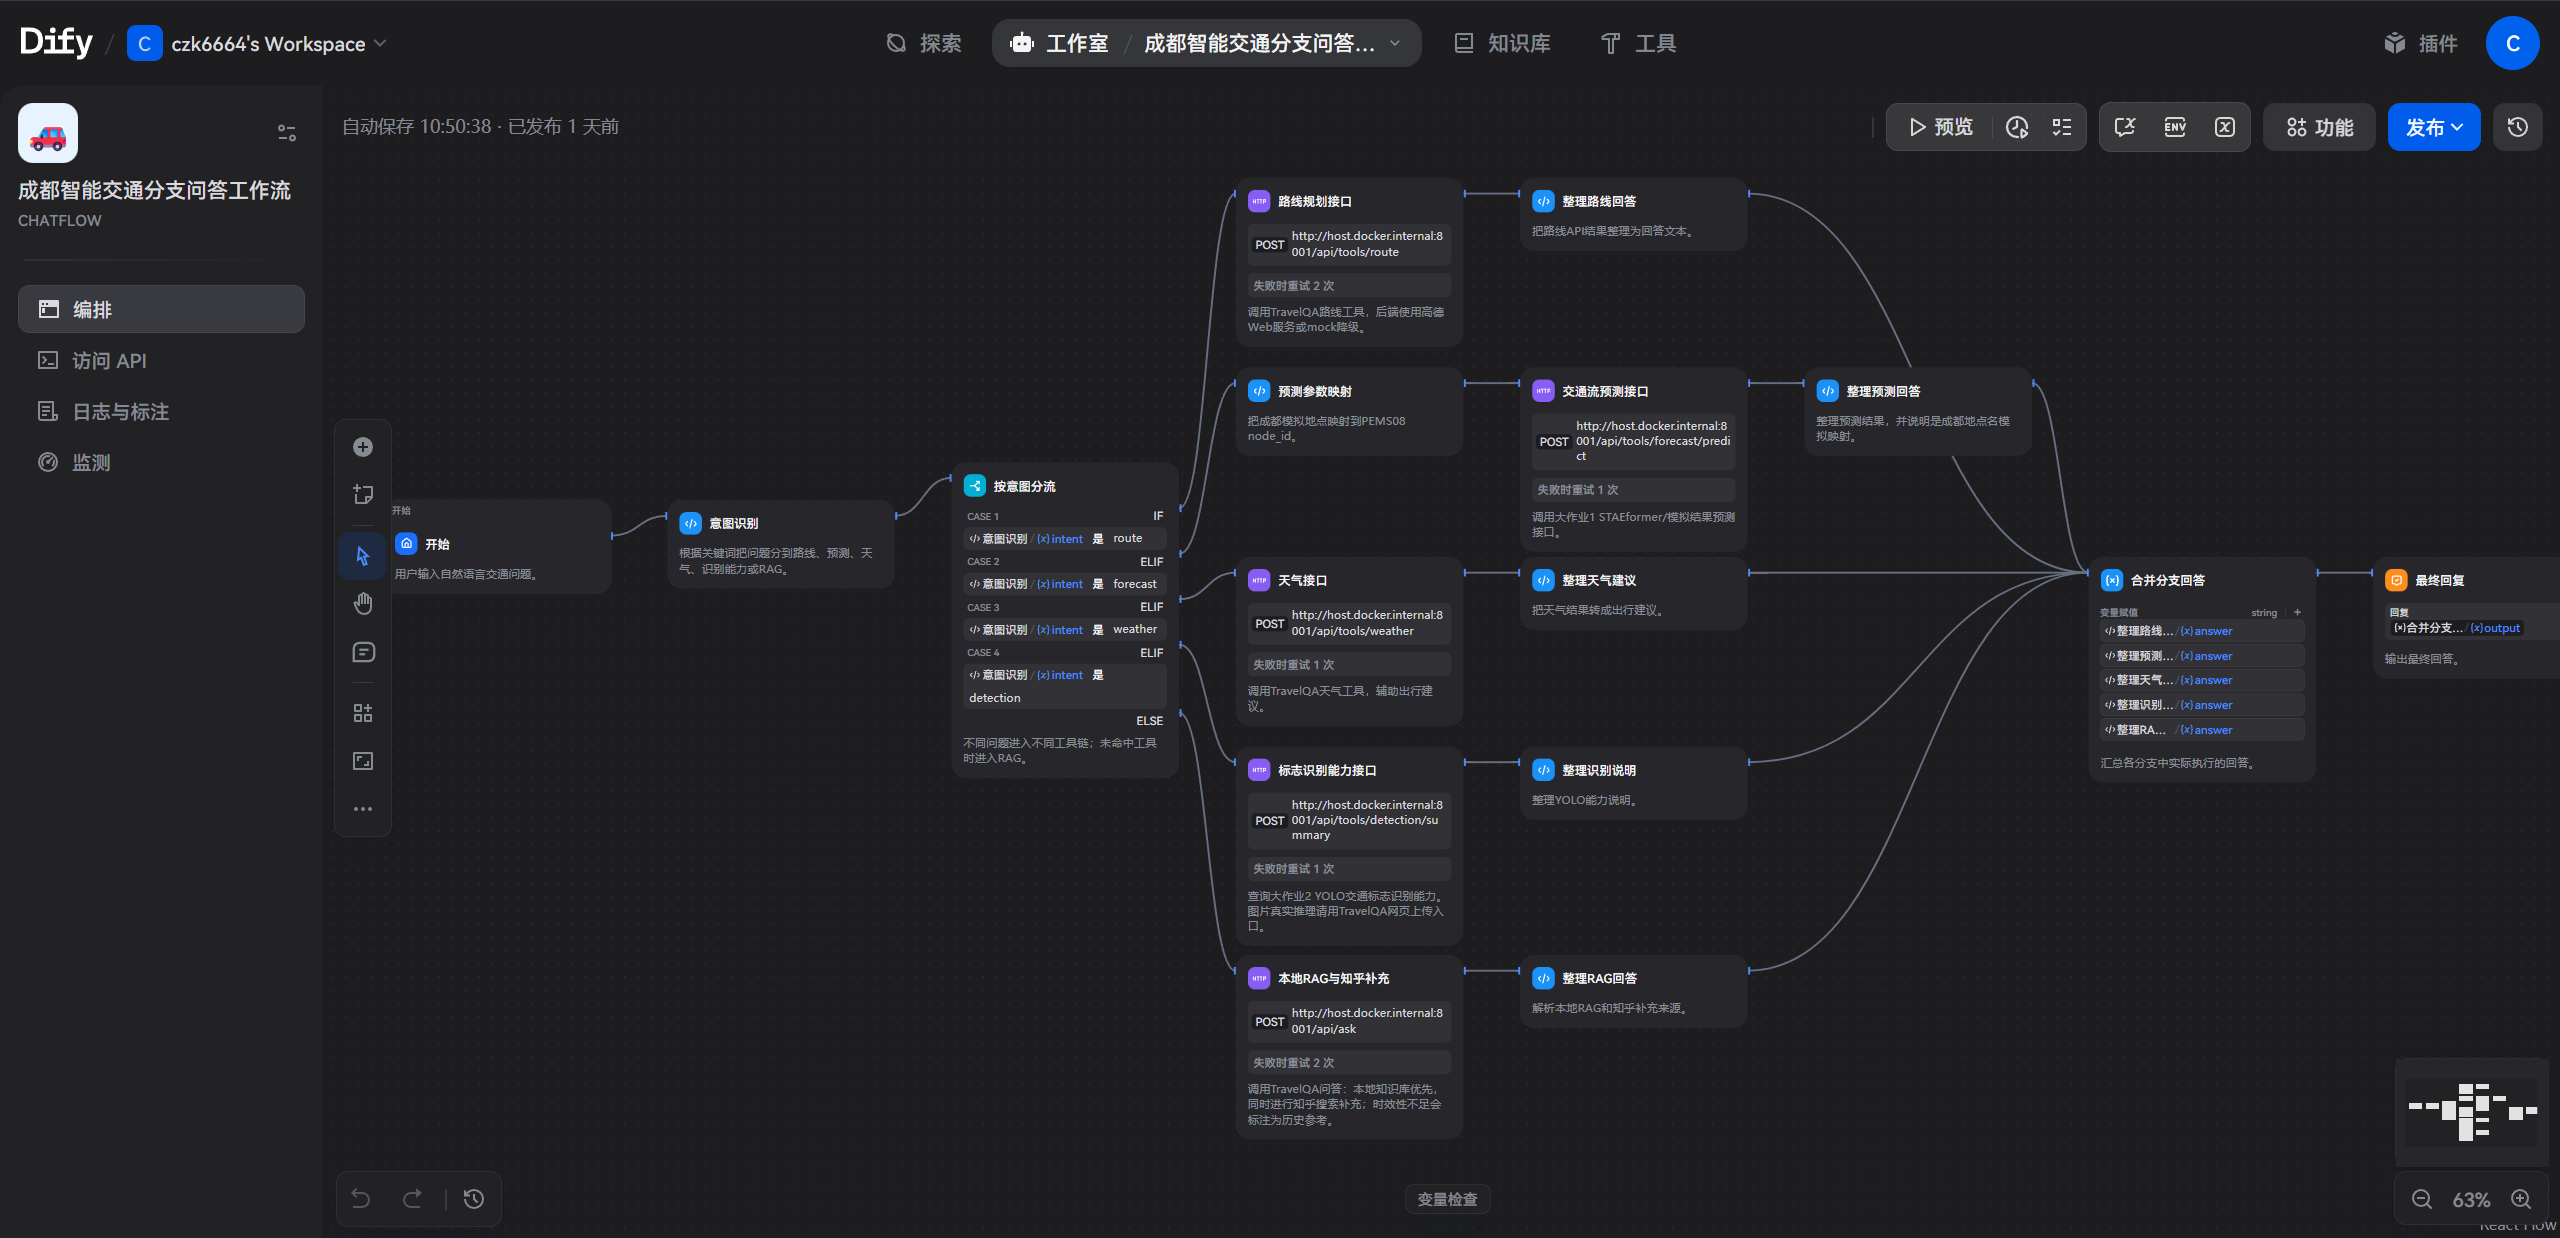
\includegraphics[width=0.96\textwidth]{figures/dify_workflow_full.png}
    \caption{Dify 工作流全景}
    \label{fig:dify-workflow-full}
\end{figure}

图\ref{fig:dify-workflow-tools} 展示了路线、交通流预测、天气和标志识别等工具分支。每个工具节点调用 TravelQA 后端的对应接口，使 Dify 工作流能够复用本地系统已有的小模型和外部 API。

\begin{figure}[H]
    \centering
    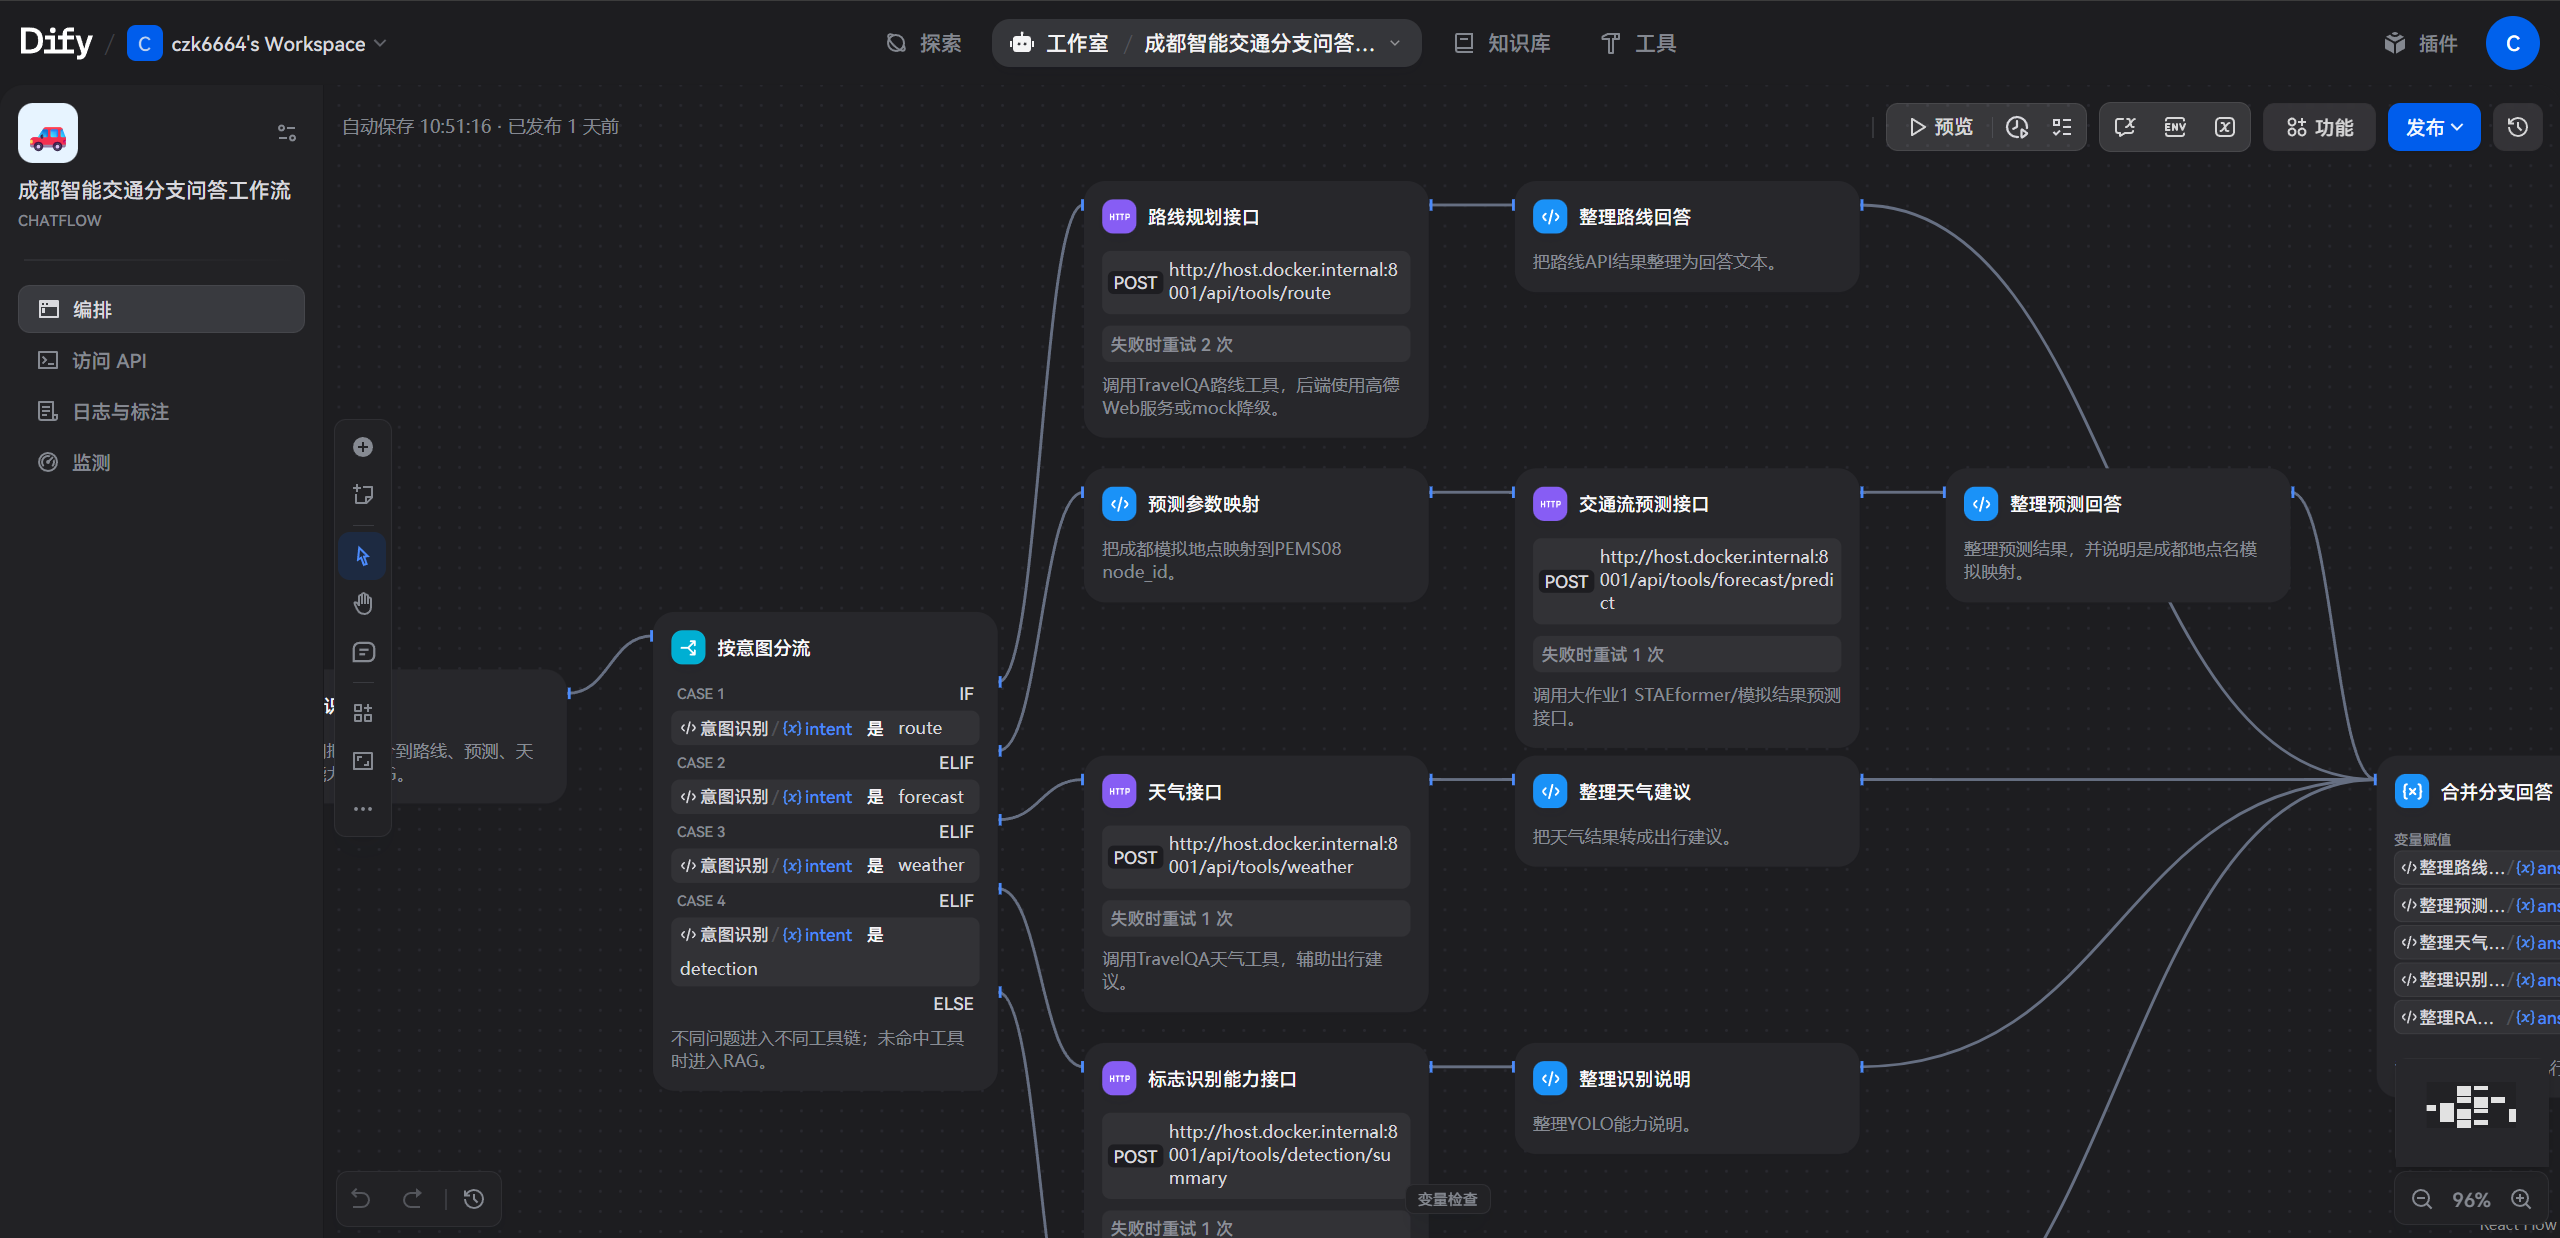
\includegraphics[width=0.96\textwidth]{figures/dify_workflow_tools.png}
    \caption{Dify 工具调用分支}
    \label{fig:dify-workflow-tools}
\end{figure}

图\ref{fig:dify-workflow-rag} 展示了天气、标志识别和本地 RAG 与知乎补充分支。对于未命中路线、预测、天气或识别的普通交通问答，工作流进入 RAG 分支，调用本地问答接口获得知识库证据和补充搜索结果。

\begin{figure}[H]
    \centering
    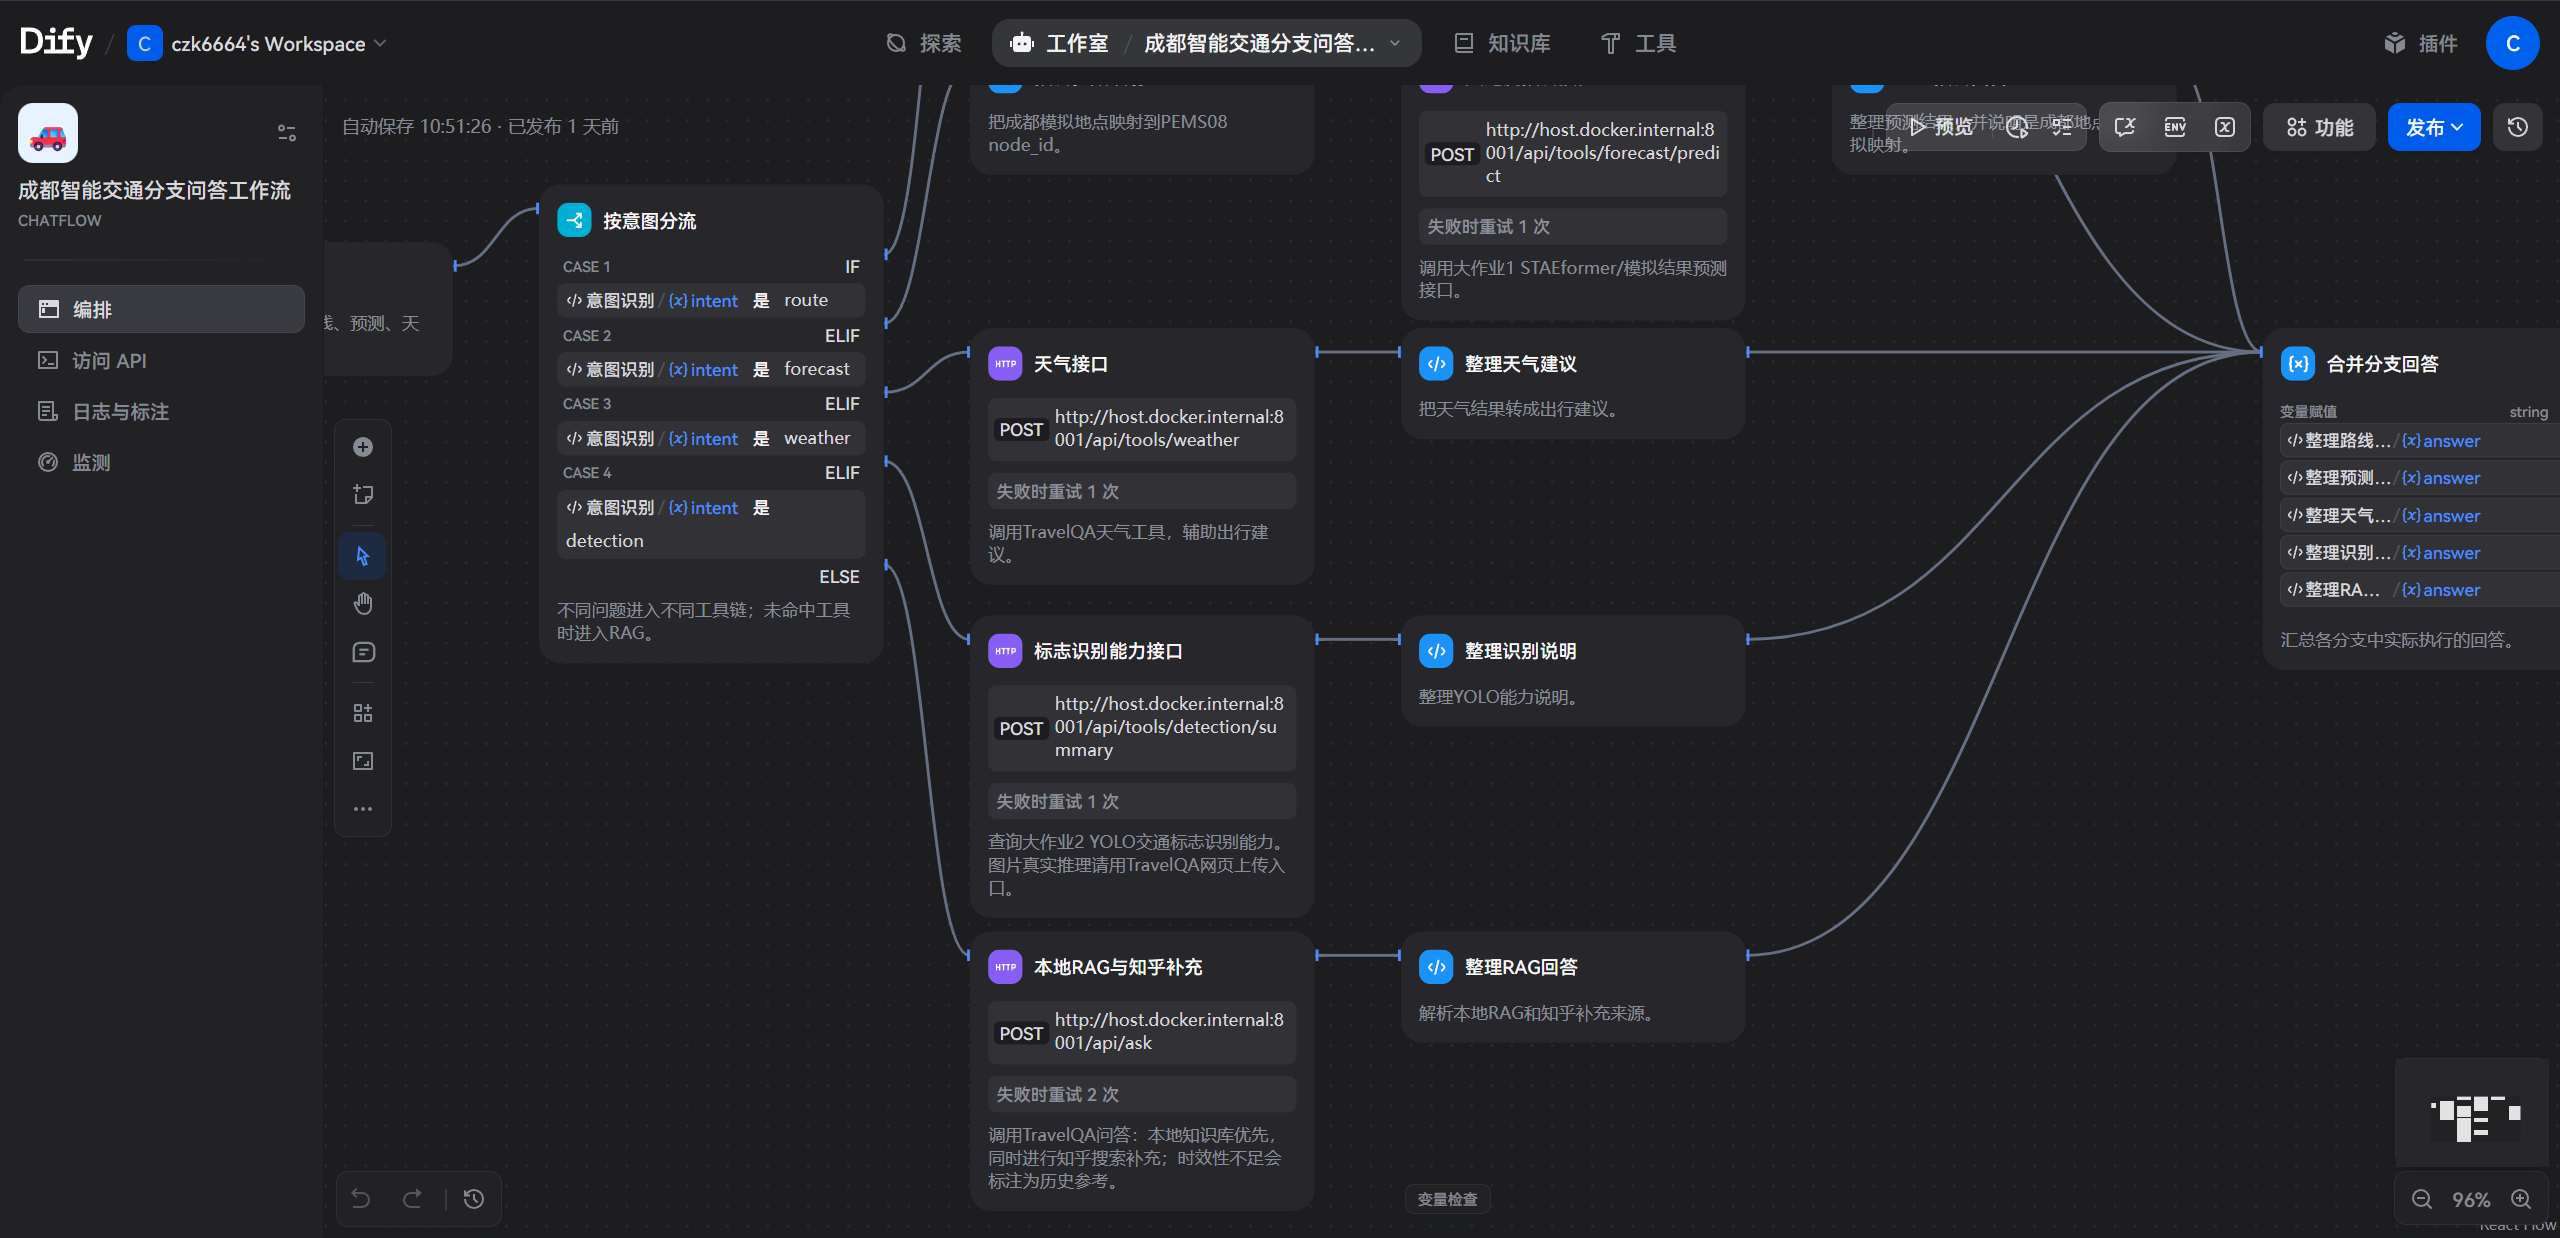
\includegraphics[width=0.96\textwidth]{figures/dify_workflow_rag.png}
    \caption{Dify RAG 与识别分支}
    \label{fig:dify-workflow-rag}
\end{figure}

\section{系统实现}
\subsection{前端实现}
前端没有使用 React/Vue 等框架，而是采用原生 HTML、CSS 与 JavaScript 实现单页应用。这个选择比较朴素，但对课程设计来说有好处：文件少、依赖少，换电脑演示时不需要额外安装前端框架。页面结构分为三栏：
\begin{itemize}
    \item 左侧控制台：运行状态、知识库状态、大模型状态、高德地图状态、Dify 状态、回答引擎切换、示例问题和图片上传。
    \item 中间问答区：展示用户输入和系统回答，回答带有意图标签。
    \item 右侧证据区：根据 panel 类型展示地图、知识片段、预测图或识别图。
\end{itemize}

前端使用统一的面板渲染函数处理结构化结果。后端返回什么类型的 panel，前端就渲染对应的证据形态。这样后续增加新工具时，前端主要补一个新的 panel 渲染器即可，不需要把问答逻辑写进页面里。

\subsection{后端实现}
后端基于 FastAPI。核心编排层负责意图识别、RAG 检索、工具调用、大模型生成和 panel 构造。我们把普通问答、地图路线、天气查询、交通流预测、图片识别和 Dify 代理都封装在同一服务中，主要是为了让前端和 Dify 工作流复用同一套接口，减少重复实现。

核心返回结构如下：
\begin{lstlisting}
{
  "intent": "route",
  "text": "回答文本",
  "sources": [],
  "tool_result": {},
  "panel": {}
}
\end{lstlisting}

\texttt{text} 用于中间问答区，\texttt{panel} 用于右侧证据与可视化区，\texttt{sources} 用于来源摘要，\texttt{tool\_result} 保留底层工具原始结构。这里特意把几个字段分开，是因为调试时经常需要判断问题出在回答生成、证据检索还是前端渲染。

后端核心编排逻辑如下。不同意图对应不同 handler，工具结果和 evidence 先生成，再由大模型或降级模板整理成面向用户的回答。

\begin{lstlisting}[language=Python]
intent = classify(query)
handler = {
    Intent.TRAFFIC_INFO: self._rag,
    Intent.TRAVEL_ADVICE: self._rag,
    Intent.WEATHER: self._weather,
    Intent.ROUTE: self._route,
    Intent.FORECAST: self._forecast,
    Intent.DETECTION: self._detection,
}[intent]
return handler(query, intent)
\end{lstlisting}

以交通流预测为例，后端会先把成都地名映射到 PEMS08 演示节点，再把预测工具结果写入 \texttt{tool\_result} 和右侧 \texttt{forecast} panel。回答文本中同步加入 \texttt{simulation\_note}，明确说明该结果是演示映射而非真实成都传感器预测。

\begin{lstlisting}[language=Python]
location, node_id = self._forecast_location_node(query)
fc = self.forecast.predict(node_id=node_id)
fc["location"] = location
fc["simulation_note"] = "成都地点名为演示用模拟映射，不是真实成都传感器数据。"
return Answer(
    intent=intent.value,
    text=text,
    evidence=f"交通流预测模型结果: {fc}",
    tool_result=fc,
    panel={"type": "forecast", "forecast": fc},
)
\end{lstlisting}

Dify 代理接口的关键点是：浏览器不直接持有 Dify App Key，而是由后端读取环境变量并调用 Dify；Dify 负责最终措辞，本地后端再针对同一问题补建右侧证据面板。这样既避免密钥暴露，也保证 Dify 模式下右侧面板不会缺失。

\begin{lstlisting}[language=Python]
resp = requests.post(
    api_base.rstrip("/") + "/chat-messages",
    headers={"Authorization": f"Bearer {api_key}"},
    json={"query": req.query, "response_mode": "blocking", "user": user},
    timeout=timeout,
)
data = resp.json()
local_context = _local_context_for_panel(req.query)
return {
    "text": data.get("answer") or "",
    "sources": local_context.get("sources") or _dify_sources(data),
    "tool_result": local_context.get("tool_result") or data,
    "panel": local_context.get("panel"),
}
\end{lstlisting}

\subsection{配置与密钥管理}
项目把普通配置与敏感密钥分开管理。普通配置用于描述工具开关、模型路径、知识库位置和成都地点映射；地图服务密钥、知乎搜索密钥和 Dify 应用密钥等敏感信息只在本地环境中读取，不写入报告正文，也不直接暴露给浏览器。

后端不会把高德 Web 服务密钥、知乎搜索密钥或 Dify 应用密钥下发到浏览器。前端只获取绘制地图所需的最小配置，其他外部服务调用都由后端代理完成。

当前 \texttt{config.yaml} 的核心结构如下。模型、RAG、外部工具和前两次大作业集成均通过配置文件声明；敏感 Key 只给出环境变量名，由本机 \texttt{.env.local} 或系统环境变量注入。这样在提交报告或复制项目时，不会把真实密钥写进源码。

\begin{lstlisting}
llm:
  provider: ollama_native
  base_url: http://127.0.0.1:11434
  model: travelqa
embedding:
  provider: sentence_transformers
  model: models/rag/bge-m3
retrieval:
  mode: hybrid
  top_k: 4
  rerank_top_k: 4
  reranker:
    provider: sentence_transformers
    model: models/rag/bge-reranker-v2-m3
tools:
  weather: {provider: amap, api_key_env: TRAVELQA_AMAP_KEY}
  route: {provider: amap, api_key_env: TRAVELQA_AMAP_KEY}
  zhihu_search: {enabled: true, secret_env: TRAVELQA_ZHIHU_API_SECRET}
integrations:
  forecast: {enabled: true, results_dir: 大作业1/results}
  detection: {enabled: true, model_path: 大作业2/.../best.pt}
\end{lstlisting}

\subsection{一键启动脚本}
为了方便课程演示，项目提供一键启动和一键停止脚本。启动脚本不只是简单启动进程，还会顺手做几项健康检查：
\begin{enumerate}
    \item 检查 Docker 是否可用，必要时启动 Docker Desktop。
    \item 启动 Dify Docker Compose 服务。
    \item 为 Dify 分配本地访问端口。
    \item 启动 TravelQA FastAPI 后端。
    \item 检查 TravelQA 和 Dify 是否正常响应。
    \item 在 Dify 容器内验证其能访问宿主机上的 TravelQA 后端。
\end{enumerate}

停止脚本会关闭 TravelQA 后端进程和 Dify Compose 容器，但不会删除知识库、模型、工作流配置和数据库数据。这样第二次演示时不用重新导入工作流或重建知识库。

\section{关键接口设计}
系统主要接口见表\ref{tab:api-list}。

\begin{table}[H]
    \caption{系统主要服务接口}
    \label{tab:api-list}
    \centering
    \small
    \begin{tabular}{p{0.24\textwidth}p{0.14\textwidth}p{0.48\textwidth}}
        \toprule[1.5pt]
        接口类别 & 方法 & 功能 \\
        \midrule[1pt]
        Web 首页 & GET & 返回三栏智能交通问答界面 \\
        健康检查 & GET & 检查后端、知识库、大模型和工具配置状态 \\
        前端配置 & GET & 返回地图绘制所需的安全前端配置 \\
        本地问答 & POST & 文本问答入口，负责意图识别、RAG、工具调用和回答生成 \\
        图片问答 & POST & 图片上传、YOLO 推理、标注图生成和大模型分析入口 \\
        Dify 状态 & GET & 检查 Dify 应用密钥和工作流服务是否可用 \\
        Dify 对话 & POST & 后端代理调用 Dify 工作流，并保持右侧证据面板一致 \\
        天气工具 & POST & 查询天气并生成出行建议 \\
        路线工具 & POST & 调用地图服务完成地点解析和路线规划 \\
        预测工具 & POST & 调用交通流预测模型获得未来一小时预测序列 \\
        识别工具 & POST & 返回交通标志识别能力说明，供工作流问答使用 \\
        静态产物 & GET & 展示上传图片、检测标注图和可视化结果 \\
        \bottomrule[1.5pt]
    \end{tabular}
\end{table}

\section{测试与验证}
\subsection{启动验证}
启动验证主要是为了避免演示时才发现某个服务没有起来。实际检查时，我们重点看 TravelQA 本地页面和 Dify 控制台两个入口；同时确认 FastAPI 后端、知识库索引、Ollama 模型服务、Dify 容器和地图配置是否能被页面识别。只要其中一个环节缺失，问答不一定完全失败，但右侧证据、地图展示或 Dify 模式就可能无法正常显示。

脚本验证通过后，至少说明以下基础链路可以正常使用：
\begin{itemize}
    \item TravelQA 三栏问答界面可以正常打开。
    \item Dify 控制台可以正常访问并运行导入的工作流。
    \item Dify 工作流能够调用本地 TravelQA 后端工具接口。
\end{itemize}

验证结束后，可以使用停止脚本关闭后端服务和 Dify 容器，同时保留本地数据与配置。

\subsection{功能测试用例}
功能测试没有追求覆盖所有真实交通场景，而是选了课程演示中最容易被问到的几类问题。测试时不只看中间有没有回答文本，还会看右侧 panel 是否同步变化：RAG 类问题要能看到证据片段，路线问题要确认高德接口被调用，预测问题要出现折线图，图片问题要能触发 YOLO 并显示标注结果。测试用例见表\ref{tab:test-cases}。

\begin{table}[H]
    \caption{核心功能测试用例}
    \label{tab:test-cases}
    \centering
    \small
    \begin{tabular}{p{0.25\textwidth}p{0.20\textwidth}p{0.42\textwidth}}
        \toprule[1.5pt]
        用户输入 & 预期意图 & 预期结果 \\
        \midrule[1pt]
        我从天府广场到春熙路怎么走？ & 路线规划 & 中间返回路线回答，右侧显示地图路线、距离、耗时和导航步骤 \\
        下雨天开车要注意什么？ & 出行建议/RAG & 本地知识库优先回答，同时展示知乎补充片段 \\
        成都尾号限行怎么规定？ & 交通信息/RAG & 展示本地依据；知乎旧结果作为历史参考，不作为当前规则 \\
        我想知道春熙路未来一小时交通流 & 交通流预测 & 春熙路映射到 node\_id=12，右侧显示预测折线图 \\
        上传交通标志图片 & 标志识别 & 调用 YOLO，右侧显示标注图、类别和置信度 \\
        切换 Dify 后提问路线问题 & Dify 工作流 & Dify 生成回答，右侧仍显示本地路线面板 \\
        \bottomrule[1.5pt]
    \end{tabular}
\end{table}

\subsection{离线评测结果}
界面截图能说明页面效果，但不方便反复检查。因此项目另外提供 \texttt{eval/run\_eval.py} 作为离线功能评测脚本。评测集 \texttt{eval/eval\_set.jsonl} 共 12 条问题，覆盖交通信息、出行建议、天气、路线、交通流预测和交通标志识别六类意图。脚本先检查 \texttt{classify(query)} 的预测意图是否正确，再调用 \texttt{TravelQAApp.ask(query)}，把回答文本和 evidence 拼接后检查人工指定的关键词是否命中。当前环境重新运行结果见表\ref{tab:offline-eval}。

\begin{table}[H]
    \caption{离线评测结果}
    \label{tab:offline-eval}
    \centering
    \begin{tabular}{p{0.34\textwidth}p{0.28\textwidth}p{0.24\textwidth}}
        \toprule[1.5pt]
        指标 & 结果 & 说明 \\
        \midrule[1pt]
        意图路由准确率 & 12/12 = 100.0\% & 六类意图均命中预期类别 \\
        关键信息命中率 & 7/7 = 100.0\% & 限行、12123、施工、车距、快处等关键词均命中 \\
        评测运行方式 & \texttt{python eval/run\_eval.py} & 不需要浏览器操作，可重复执行 \\
        \bottomrule[1.5pt]
    \end{tabular}
\end{table}

在基础 12 条评测外，项目进一步加入 \texttt{eval/intent\_compare\_set.jsonl}，扩展到 18 条意图分类问题，覆盖``从 A 到 B 堵不堵''、``没有预测文件能否直接说准确率''、``上传图片后能否检测标志''等更接近真实问法的样例。脚本 \texttt{eval/run\_intent\_compare.py} 会先运行本地规则分类器；若本机 Ollama 中的 \texttt{travelqa} 模型可用，还会用同一 few-shot prompt 执行 LLM 分类对比。当前验收环境中 Ollama 服务未启动，因此 LLM 分类分支记录为 \texttt{not\_run}。这个结果没有删掉，因为它正好说明当前评测环境下只验证了规则路由，LLM 分类还需要在模型服务启动后再补测。规则路由结果见表\ref{tab:intent-extended}。

\begin{table}[H]
    \caption{扩展意图分类评测}
    \label{tab:intent-extended}
    \centering
    \small
    \begin{tabular}{p{0.30\textwidth}p{0.24\textwidth}p{0.30\textwidth}}
        \toprule[1.5pt]
        指标 & 结果 & 说明 \\
        \midrule[1pt]
        扩展样本数 & 18 条 & 六类意图，每类含边界问法 \\
        规则路由准确率 & 18/18 = 100.0\% & 已修正``堵不堵''实时路线漏判 \\
        LLM few-shot 分类 & 当前未运行 & Ollama 未启动，脚本保留 prompt 与接口 \\
        输出文件 & 结果 JSON & 保存每条规则预测与 LLM 状态 \\
        \bottomrule[1.5pt]
    \end{tabular}
\end{table}

RAG 这部分我们更关心证据有没有找对。交通类问题里，路名、时间、政策关键词都很关键；同样是交通管制，公告里的道路或生效时间只要错一个，后面的回答就会跟着偏。因此这里单独准备了 RAG 评测脚本和标注集。评测集包含 20 条人工标注查询，每条给出应命中的官方公告或法规标题片段；脚本把检索结果的来源标题与标注片段匹配，计算 Top-1、Top-3 和 Top-5 来源命中率。这个评测只看``是否召回正确来源''，不把大模型最终生成文本纳入评分，因此更适合单独检查检索模块。结果见表\ref{tab:rag-eval}。

\begin{table}[H]
    \caption{RAG 来源 Top-K 命中率}
    \label{tab:rag-eval}
    \centering
    \begin{tabular}{p{0.28\textwidth}p{0.28\textwidth}p{0.30\textwidth}}
        \toprule[1.5pt]
        指标 & 结果 & 说明 \\
        \midrule[1pt]
        评测样本数 & 20 条 & 覆盖 15 条交管公告、3 条法规和 2 条泛化查询 \\
        Top-1 命中率 & 20/20 = 100.0\% & 正确来源均排在第 1 位 \\
        Top-3 命中率 & 20/20 = 100.0\% & 正确来源均进入前 3 \\
        Top-5 命中率 & 20/20 = 100.0\% & 正确来源均进入前 5 \\
        输出文件 & RAG 评测 JSON & 保存每条问题的命中排名和 Top-5 标题 \\
        \bottomrule[1.5pt]
    \end{tabular}
\end{table}

为了看 Hybrid Search 和 Reranker 是否真的起作用，脚本同时输出了小规模消融结果。表\ref{tab:rag-ablation} 显示，在同一 20 条评测集上，当前方案 Top-1 命中 20/20；去掉 Reranker 后 Hybrid 检索 Top-1 降为 19/20；仅使用向量检索且不重排时 Top-1 降为 18/20。这个结果也符合调试时的观察：路名、区域名和公告标题比较多时，只靠语义相似并不保险，BM25 与 Reranker 对首位排序更有帮助。

\begin{table}[H]
    \caption{RAG 检索消融结果}
    \label{tab:rag-ablation}
    \centering
    \small
    \begin{tabular}{p{0.34\textwidth}p{0.18\textwidth}p{0.18\textwidth}p{0.18\textwidth}}
        \toprule[1.5pt]
        检索方案 & Top-1 & Top-3 & Top-5 \\
        \midrule[1pt]
        Hybrid + Reranker & 20/20 & 20/20 & 20/20 \\
        Hybrid，无 Reranker & 19/20 & 19/20 & 19/20 \\
        纯向量，无 Reranker & 18/20 & 20/20 & 20/20 \\
        \bottomrule[1.5pt]
    \end{tabular}
\end{table}

考虑到 20 条来源命中率评测相对友好，项目又加入了 RAG 压力集标注文件和配套脚本。压力集包含 8 条可回答问题和 4 条负例问题：可回答问题继续要求 Top-K 命中正确来源；负例问题包括广州、北京、成都不存在路名和强时效活动问题，要求检索结果不要出现精确错误匹配，且最高相似分低于阈值。这个压力集保留了失败情况，方便后面定位边界问题。结果见表\ref{tab:rag-stress}。

\begin{table}[H]
    \caption{RAG 压力集与边界评测}
    \label{tab:rag-stress}
    \centering
    \small
    \begin{tabular}{p{0.34\textwidth}p{0.22\textwidth}p{0.30\textwidth}}
        \toprule[1.5pt]
        指标 & 结果 & 说明 \\
        \midrule[1pt]
        可回答正例 Top-1/3/5 & 8/8，8/8，8/8 & 官方公告和法规问题均命中正确来源 \\
        负例边界通过率 & 2/4 = 50.0\% & 广州、北京问题通过；成都近似时效问题仍会召回相近公告 \\
        总通过率 & 10/12 = 83.3\% & 比友好集更能暴露边界缺口 \\
        输出文件 & 压力集结果 JSON & 保存每条 Top-5 标题和分数 \\
        \bottomrule[1.5pt]
    \end{tabular}
\end{table}

当前 RAG 评测仍以来源召回和边界检索为主，适合验证公告和法规是否被正确召回，以及知识库对外地或未覆盖问题是否容易误召回。它还不能等价为最终答案事实性评测。Top-K 命中只能说明依据被找到了，不代表模型一定引用得准确。若要进一步评估回答本身，还需要人工标注标准答案，并加入回答准确率、引用正确率和有无 RAG 的生成质量对比。压力集暴露出的主要问题是：当问题仍含有``成都''和``交通管制''等强领域词，但具体事件不在知识库中时，检索器会返回语义相近的成都公告。因此，后续应在回答层加入地域、事件名和发布时间守门规则，对最高分低或实体不一致的结果明确提示``知识库未覆盖该问题''。

\subsection{端到端延迟测试}
延迟测试主要服务于课堂演示体验，而不是严格性能压测。在当前本地环境中，使用 \texttt{TravelQAApp.ask()} 对六类典型问题各测试一次，得到表\ref{tab:latency}。该测试包含意图识别、检索或工具调用、模型组织回答与 panel 构造，不包含浏览器渲染时间。

\begin{table}[H]
    \caption{典型问题端到端响应时间}
    \label{tab:latency}
    \centering
    \small
    \begin{tabular}{p{0.26\textwidth}p{0.22\textwidth}p{0.20\textwidth}p{0.16\textwidth}}
        \toprule[1.5pt]
        问题类型 & 识别意图 & 响应时间 / s & panel 类型 \\
        \midrule[1pt]
        尾号限行 RAG & traffic-info & 2.934 & rag \\
        雨天出行建议 & travel-advice & 3.215 & rag \\
        天气问答 & weather & 2.374 & 无右侧 panel \\
        路线规划 & route & 3.258 & route \\
        交通流预测 & forecast & 2.618 & forecast \\
        识别能力问答 & detection & 2.054 & detection \\
        \bottomrule[1.5pt]
    \end{tabular}
\end{table}

这组延迟测试只能说明本机环境下单次请求大致能跑通。RAG 和路线规划略慢，耗时来源不一样：RAG 需要完成向量检索、BM25 重排和证据整理，路线规划则依赖高德 API 的返回速度。预测和识别能力问答主要读取本地结果文件，因此耗时更低。Dify 模式还会多一层工作流调用，实际体验会受容器和网络状态影响。这里没有做高并发压测，测试更接近单人课堂演示场景；如果要部署到真实并发环境，还需要使用 \texttt{locust}、\texttt{wrk} 或 \texttt{pytest-benchmark} 分别统计模型推理、RAG 检索和外部 API 调用耗时。

\subsection{界面与运行截图}
图\ref{fig:ui-route-tianfu} 展示了从天府广场到春熙路的路径规划结果。中间问答区给出路线摘要和主要步骤，右侧面板调用高德地图显示起点、终点、路径轨迹、距离和预计耗时。

\begin{figure}[H]
    \centering
    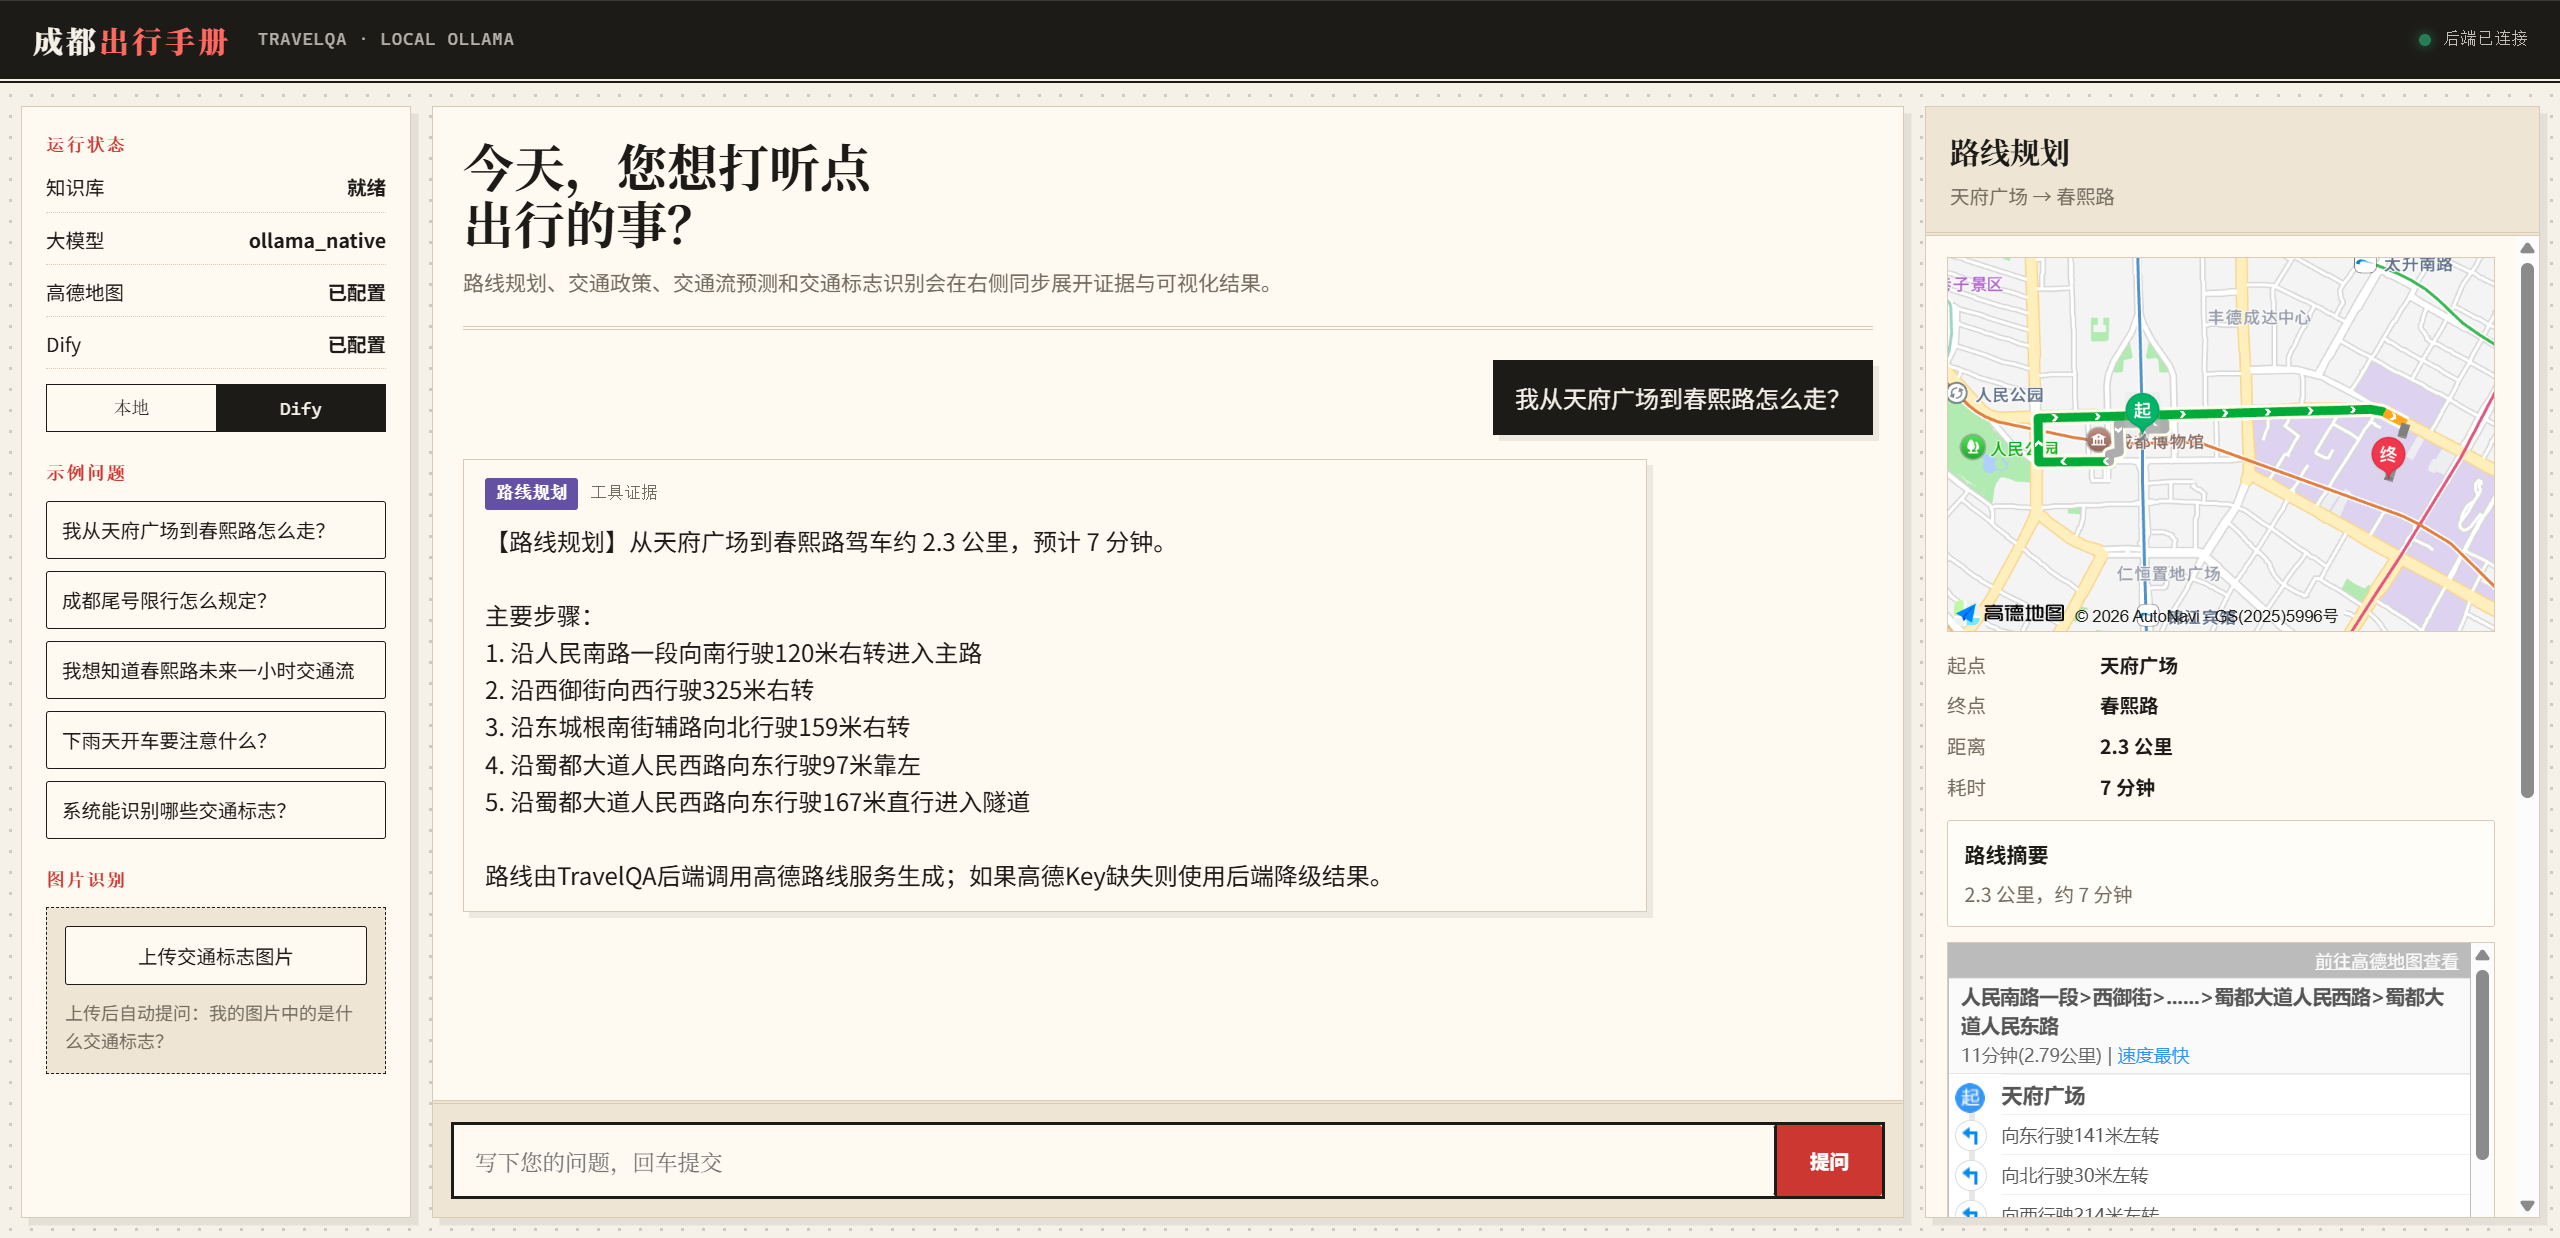
\includegraphics[width=0.96\textwidth]{figures/ui_route_tianfu.png}
    \caption{天府广场到春熙路路线规划界面}
    \label{fig:ui-route-tianfu}
\end{figure}

图\ref{fig:ui-route-wanxiang} 展示了从西南交大犀浦校区到万象城的另一条路线规划。该截图用于说明系统不只依赖固定示例，也可以根据自然语言抽取起终点，并生成路线证据面板。

\begin{figure}[H]
    \centering
    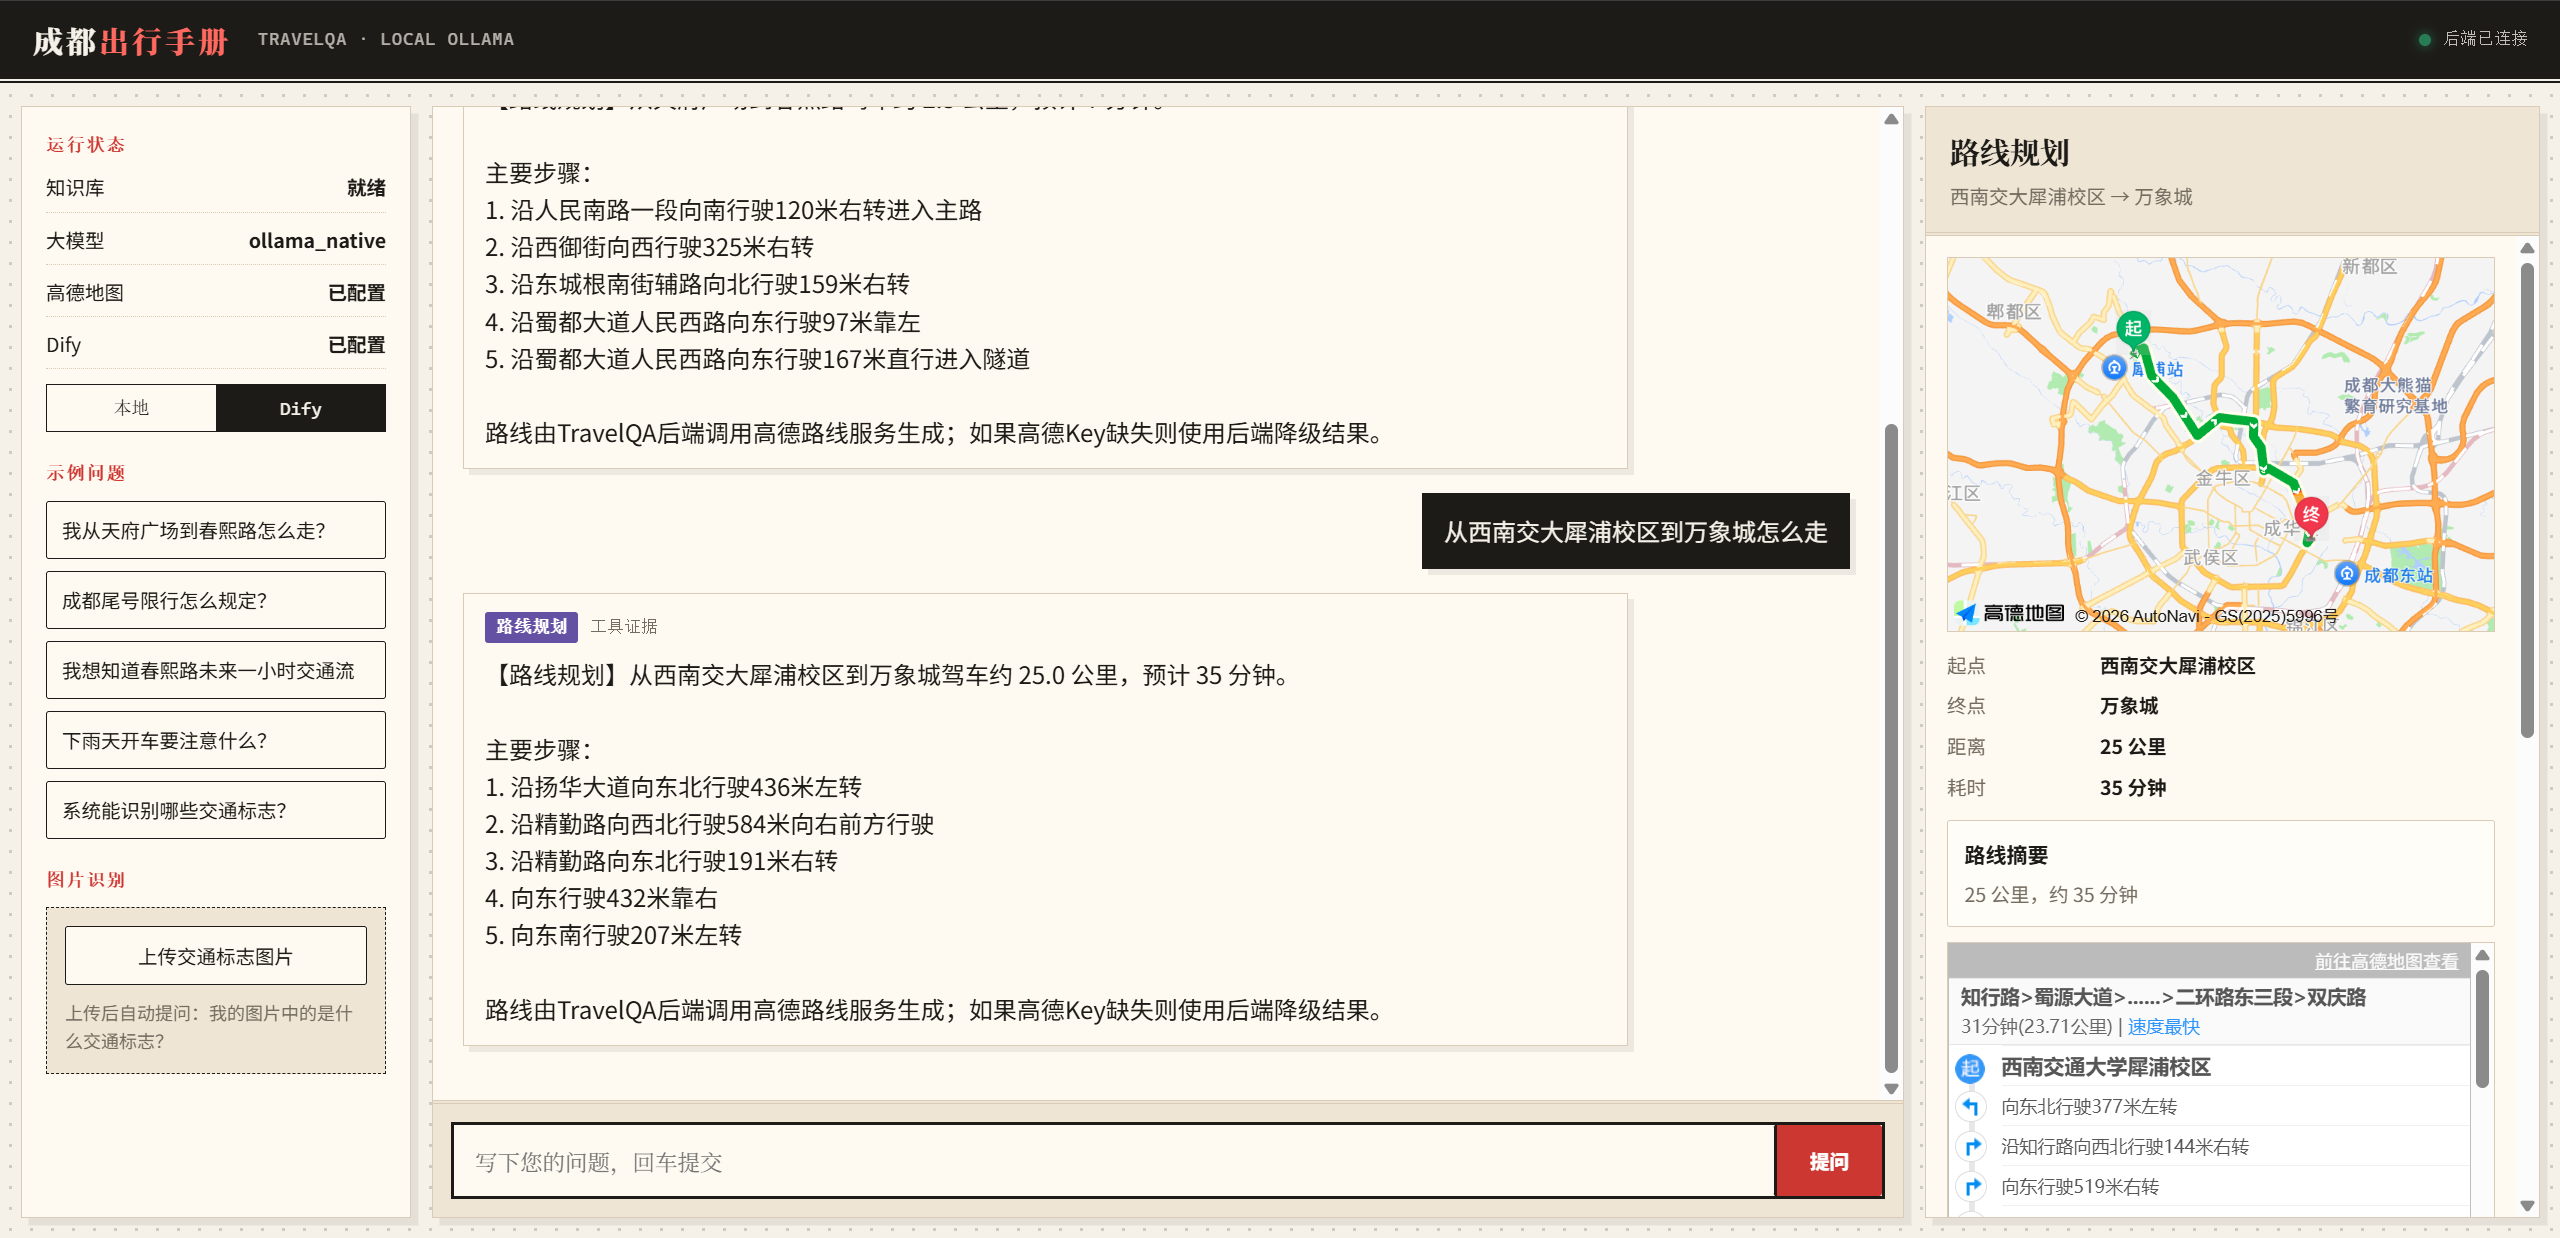
\includegraphics[width=0.96\textwidth]{figures/ui_route_wanxiang.png}
    \caption{西南交大犀浦校区到万象城路线规划界面}
    \label{fig:ui-route-wanxiang}
\end{figure}

图\ref{fig:ui-rag-zhihu} 展示了尾号限行类强时效问题的回答。由于本地知识库未命中当前有效依据，系统将知乎搜索结果作为参考展示，并在回答中明确说明其仅供参考、不代表官方结论。

\begin{figure}[H]
    \centering
    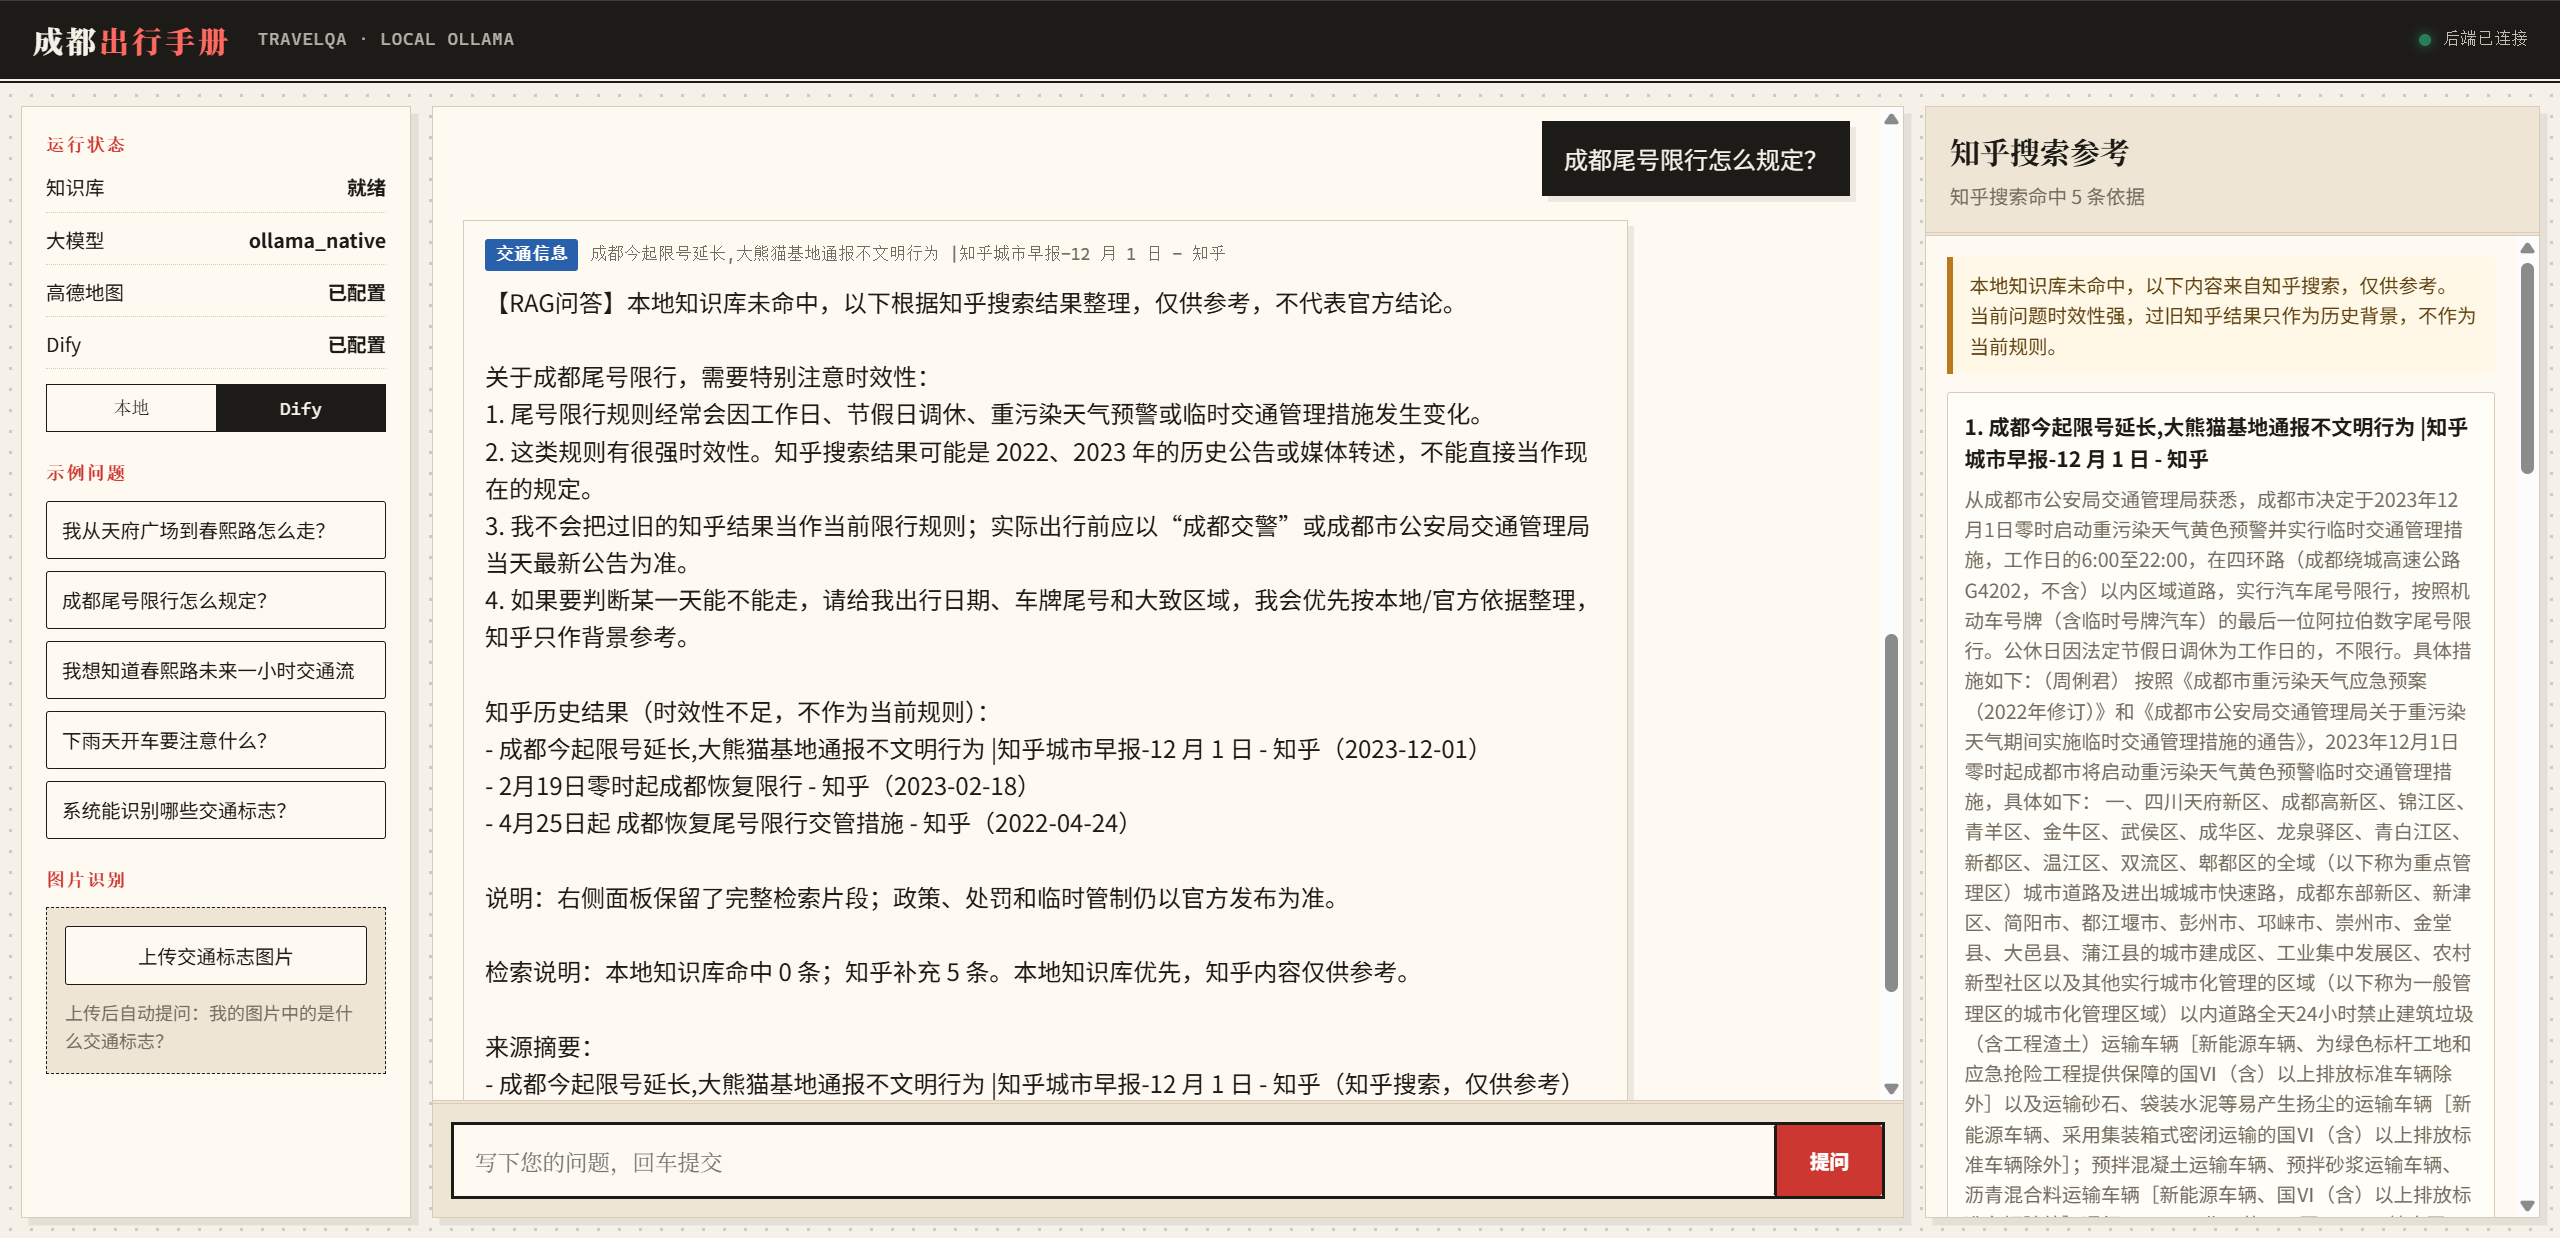
\includegraphics[width=0.96\textwidth]{figures/ui_rag_zhihu.png}
    \caption{尾号限行问题的知乎补充参考界面}
    \label{fig:ui-rag-zhihu}
\end{figure}

图\ref{fig:ui-rag-local} 展示了本地知识库命中的 RAG 问答。用户询问熊猫基地相关交通管理问题时，系统优先使用本地公告片段，并在右侧展示来源标题、发布时间、正文摘要和来源信息。

\begin{figure}[H]
    \centering
    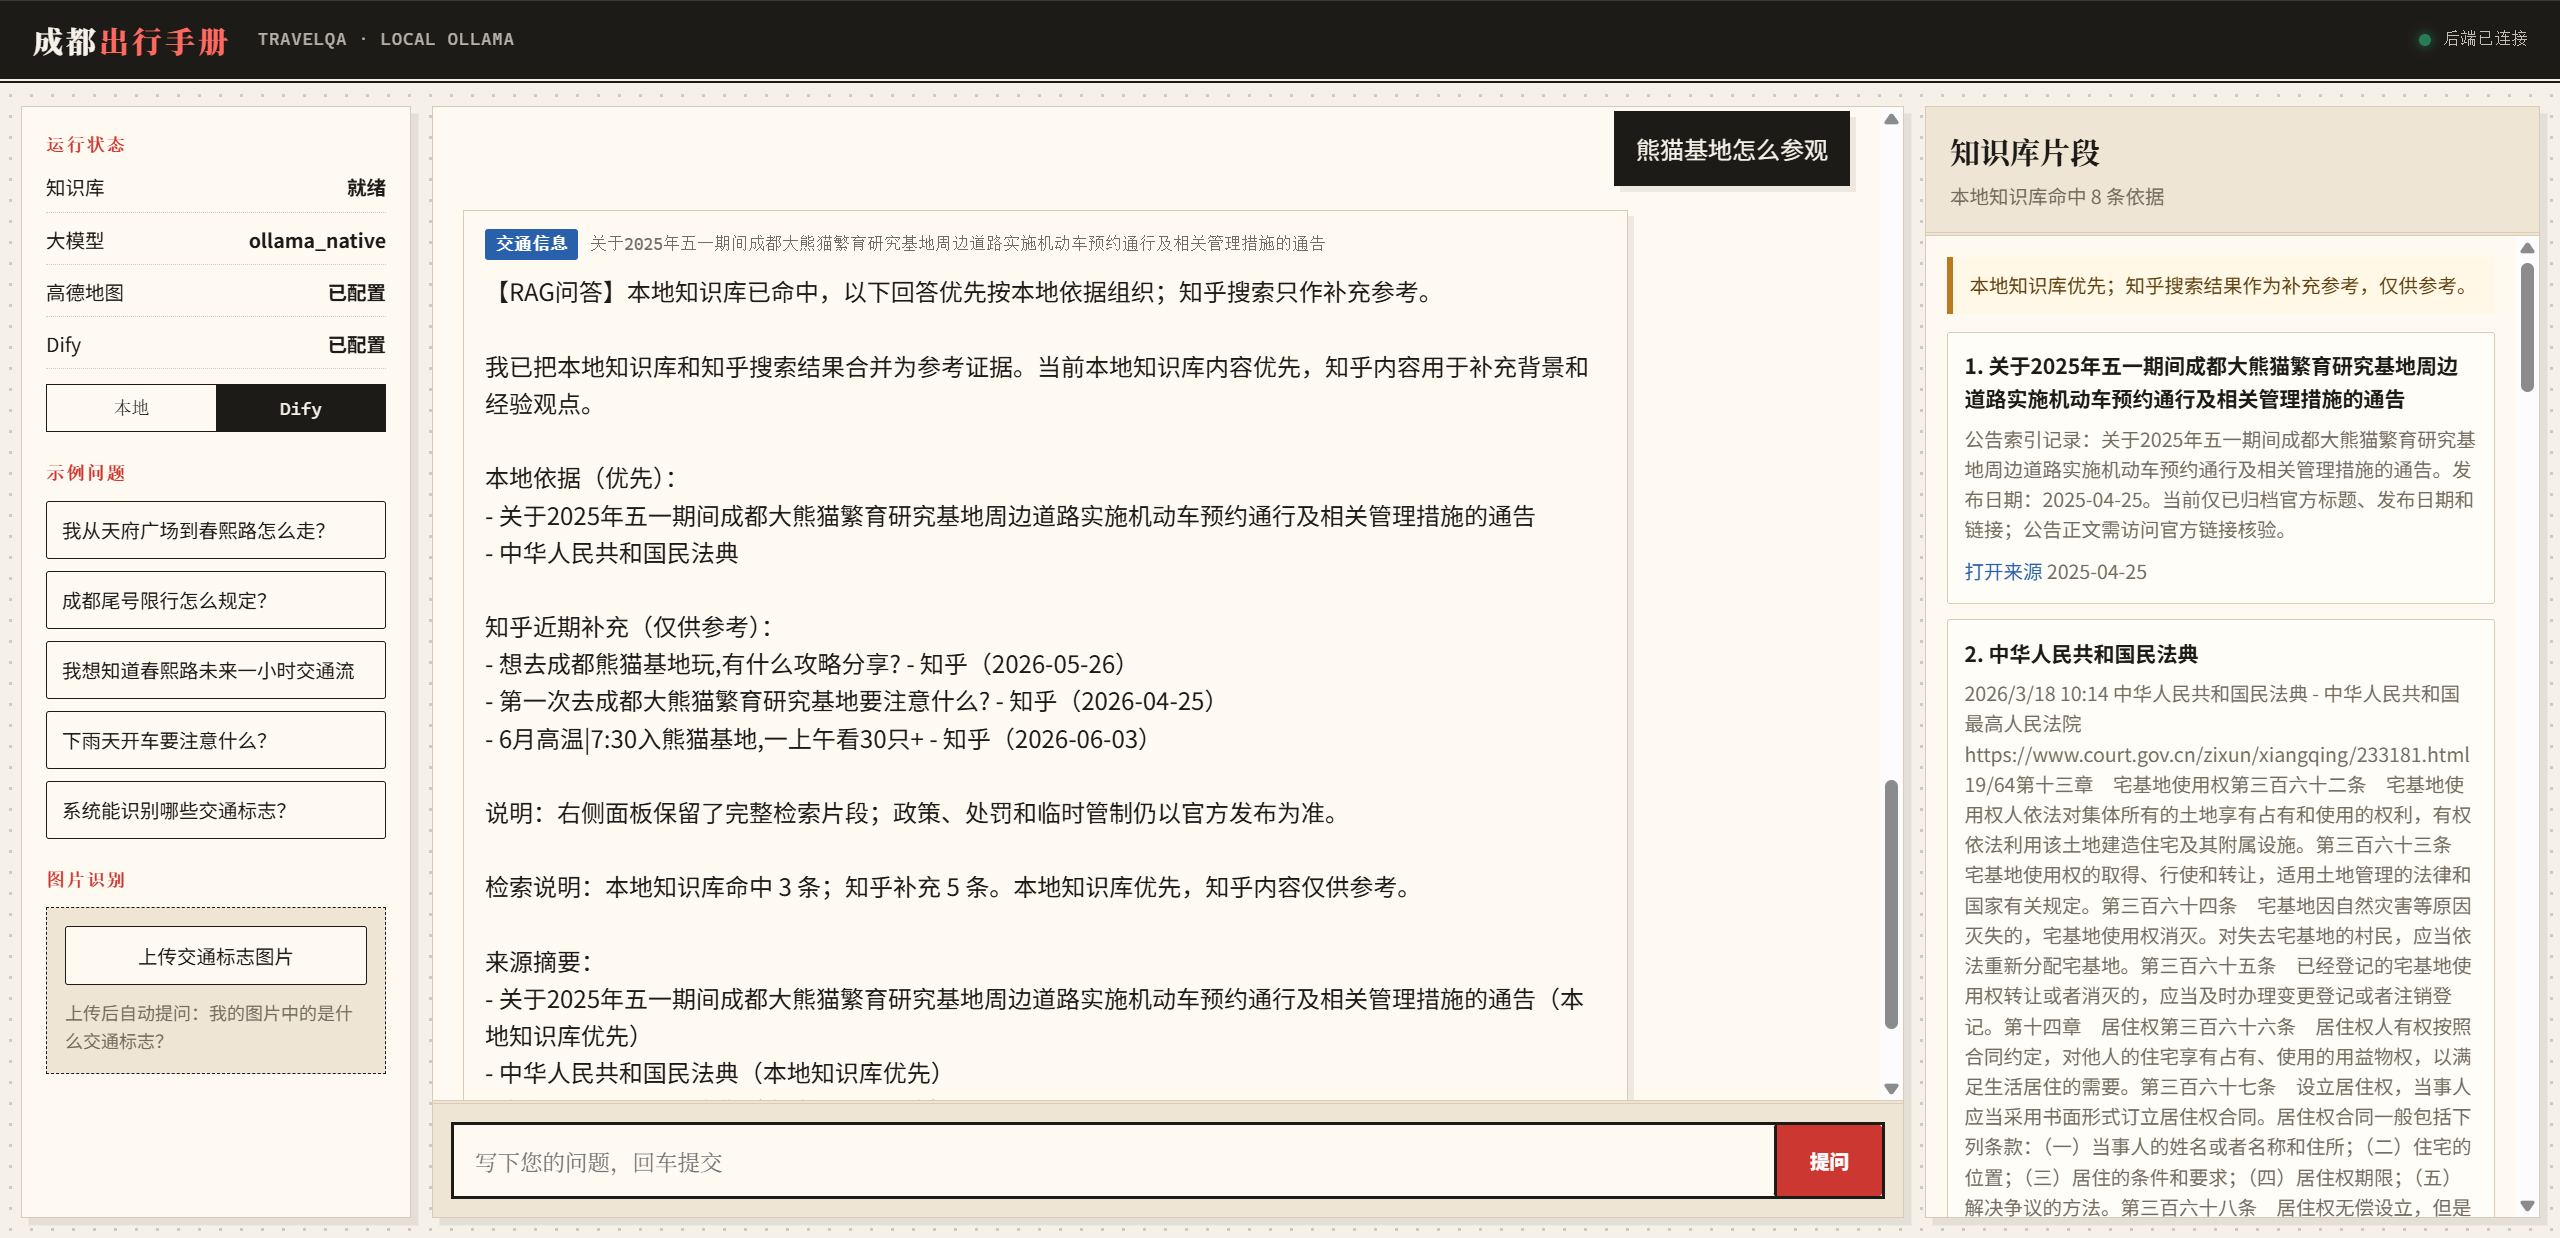
\includegraphics[width=0.96\textwidth]{figures/ui_rag_local.png}
    \caption{本地 RAG 命中与证据片段展示}
    \label{fig:ui-rag-local}
\end{figure}

图\ref{fig:ui-forecast} 展示了交通流预测问答。系统将春熙路映射到 PEMS08 的演示节点，调用 STAEformer 预测未来 60 分钟交通流，并在右侧绘制趋势曲线和各时间步预测值。

\begin{figure}[H]
    \centering
    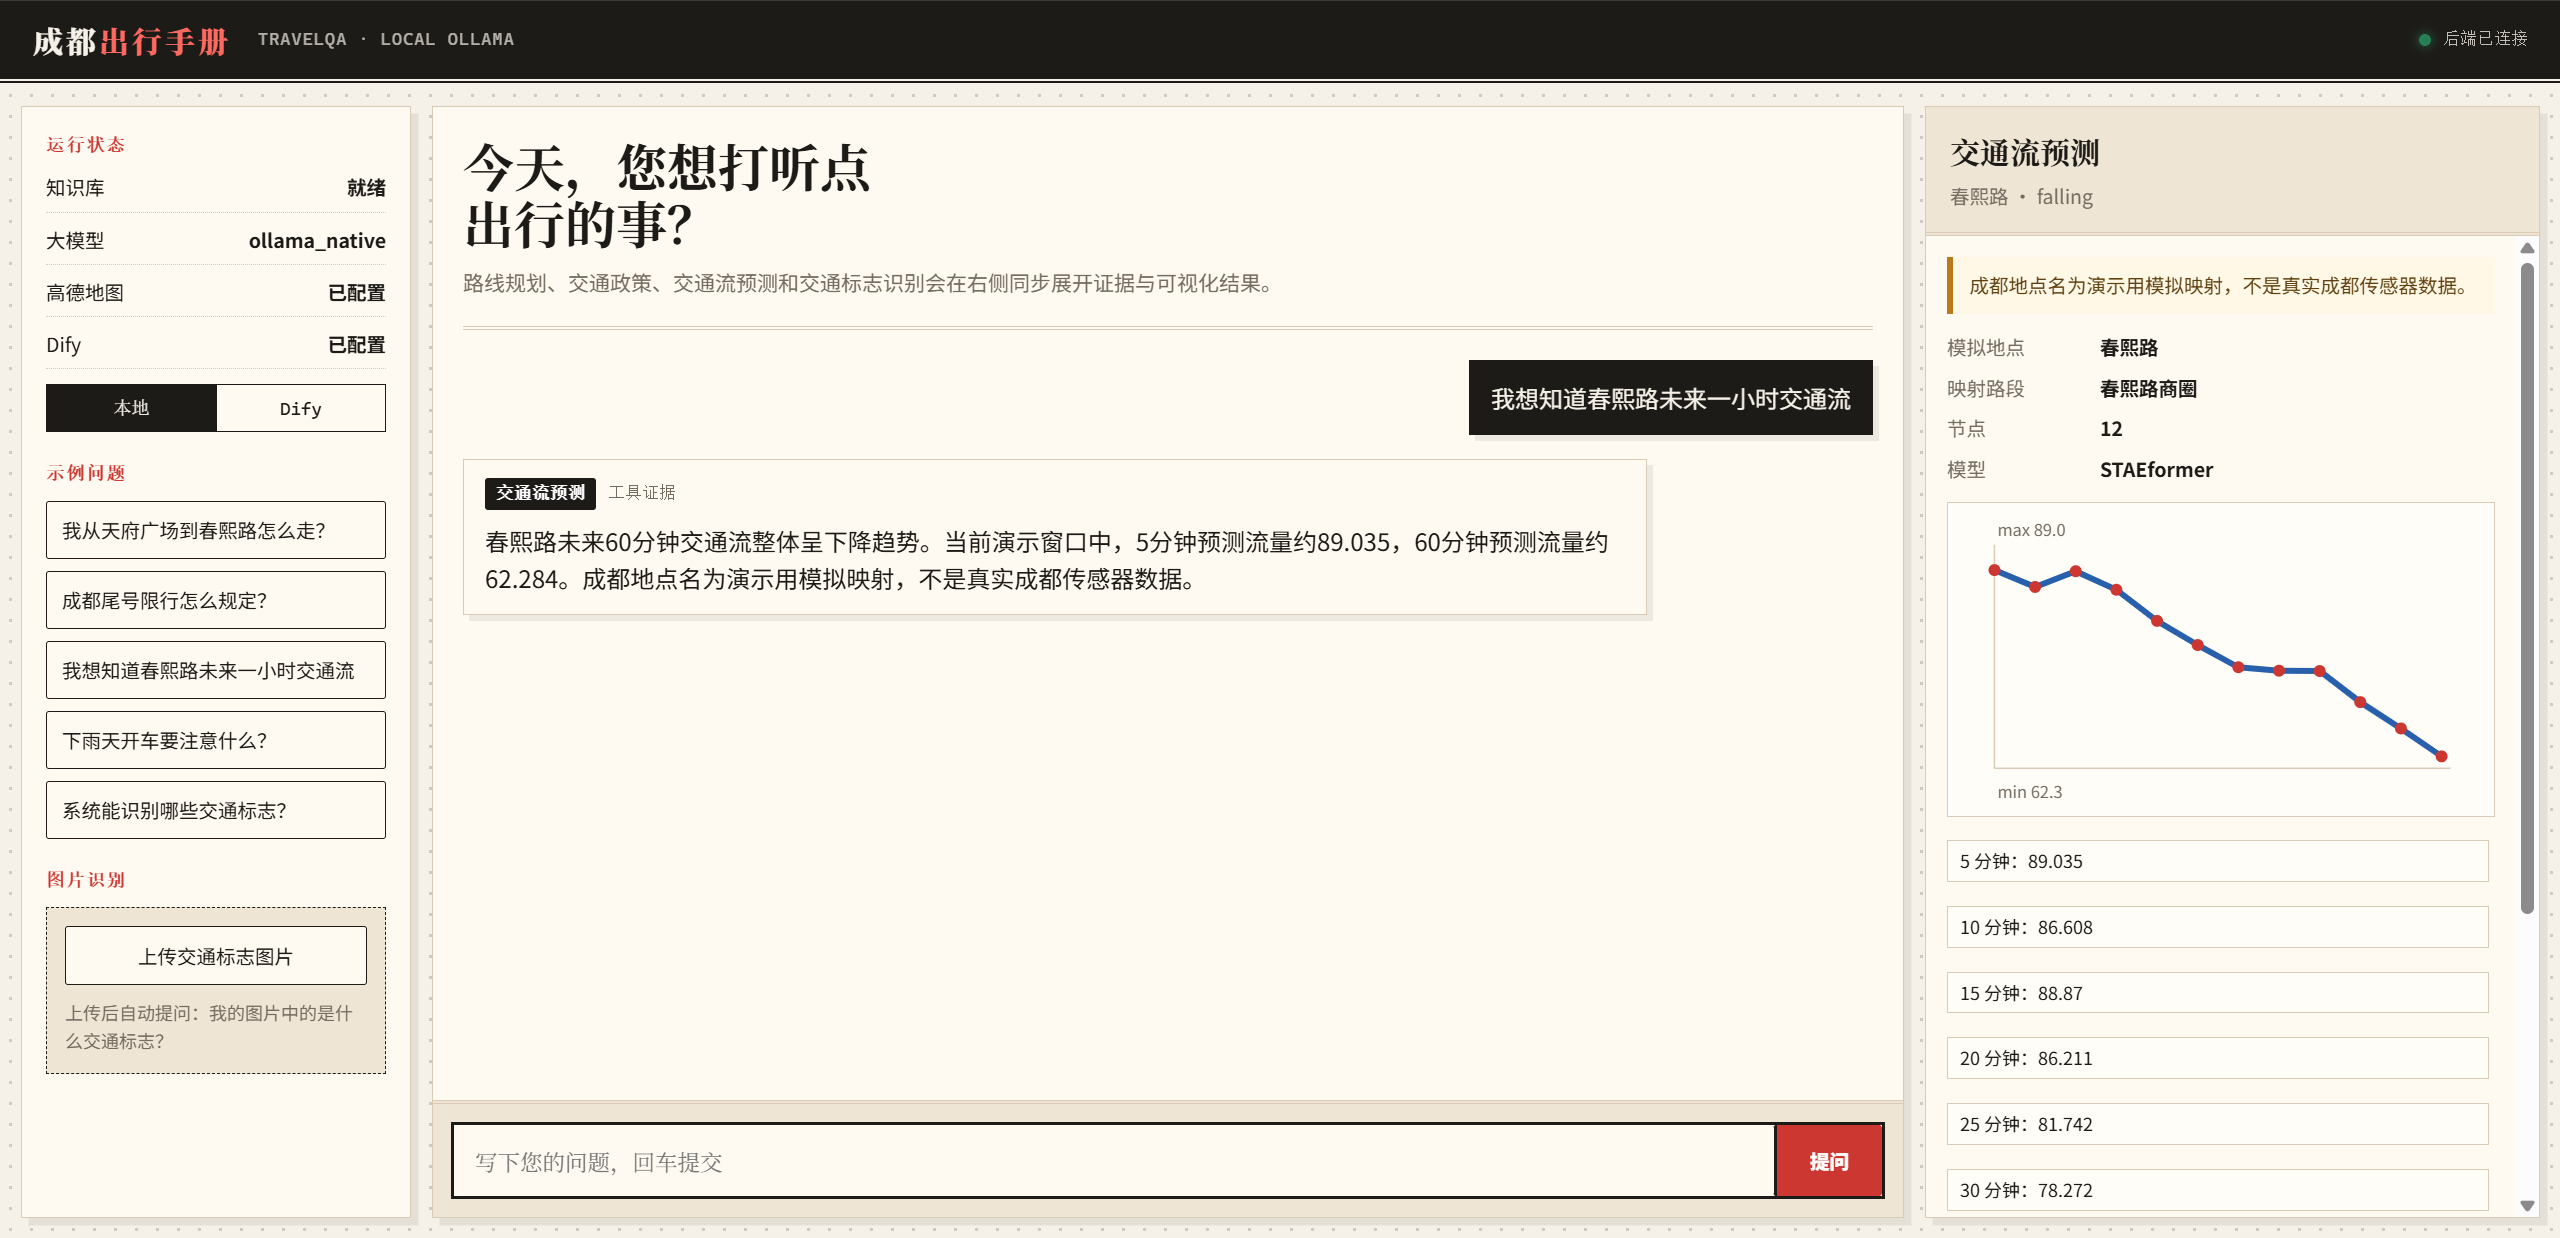
\includegraphics[width=0.96\textwidth]{figures/ui_forecast.png}
    \caption{春熙路未来一小时交通流预测界面}
    \label{fig:ui-forecast}
\end{figure}

图\ref{fig:ui-detection-result} 展示了交通标志图片识别功能。用户上传``禁止驶入''标志图片后，系统在中间问答区给出识别结论，右侧面板展示标注图、类别、置信度和边界框坐标。这也是三栏界面设计的一个典型例子：中间回答问题，右侧展示工具证据。

\begin{figure}[H]
    \centering
    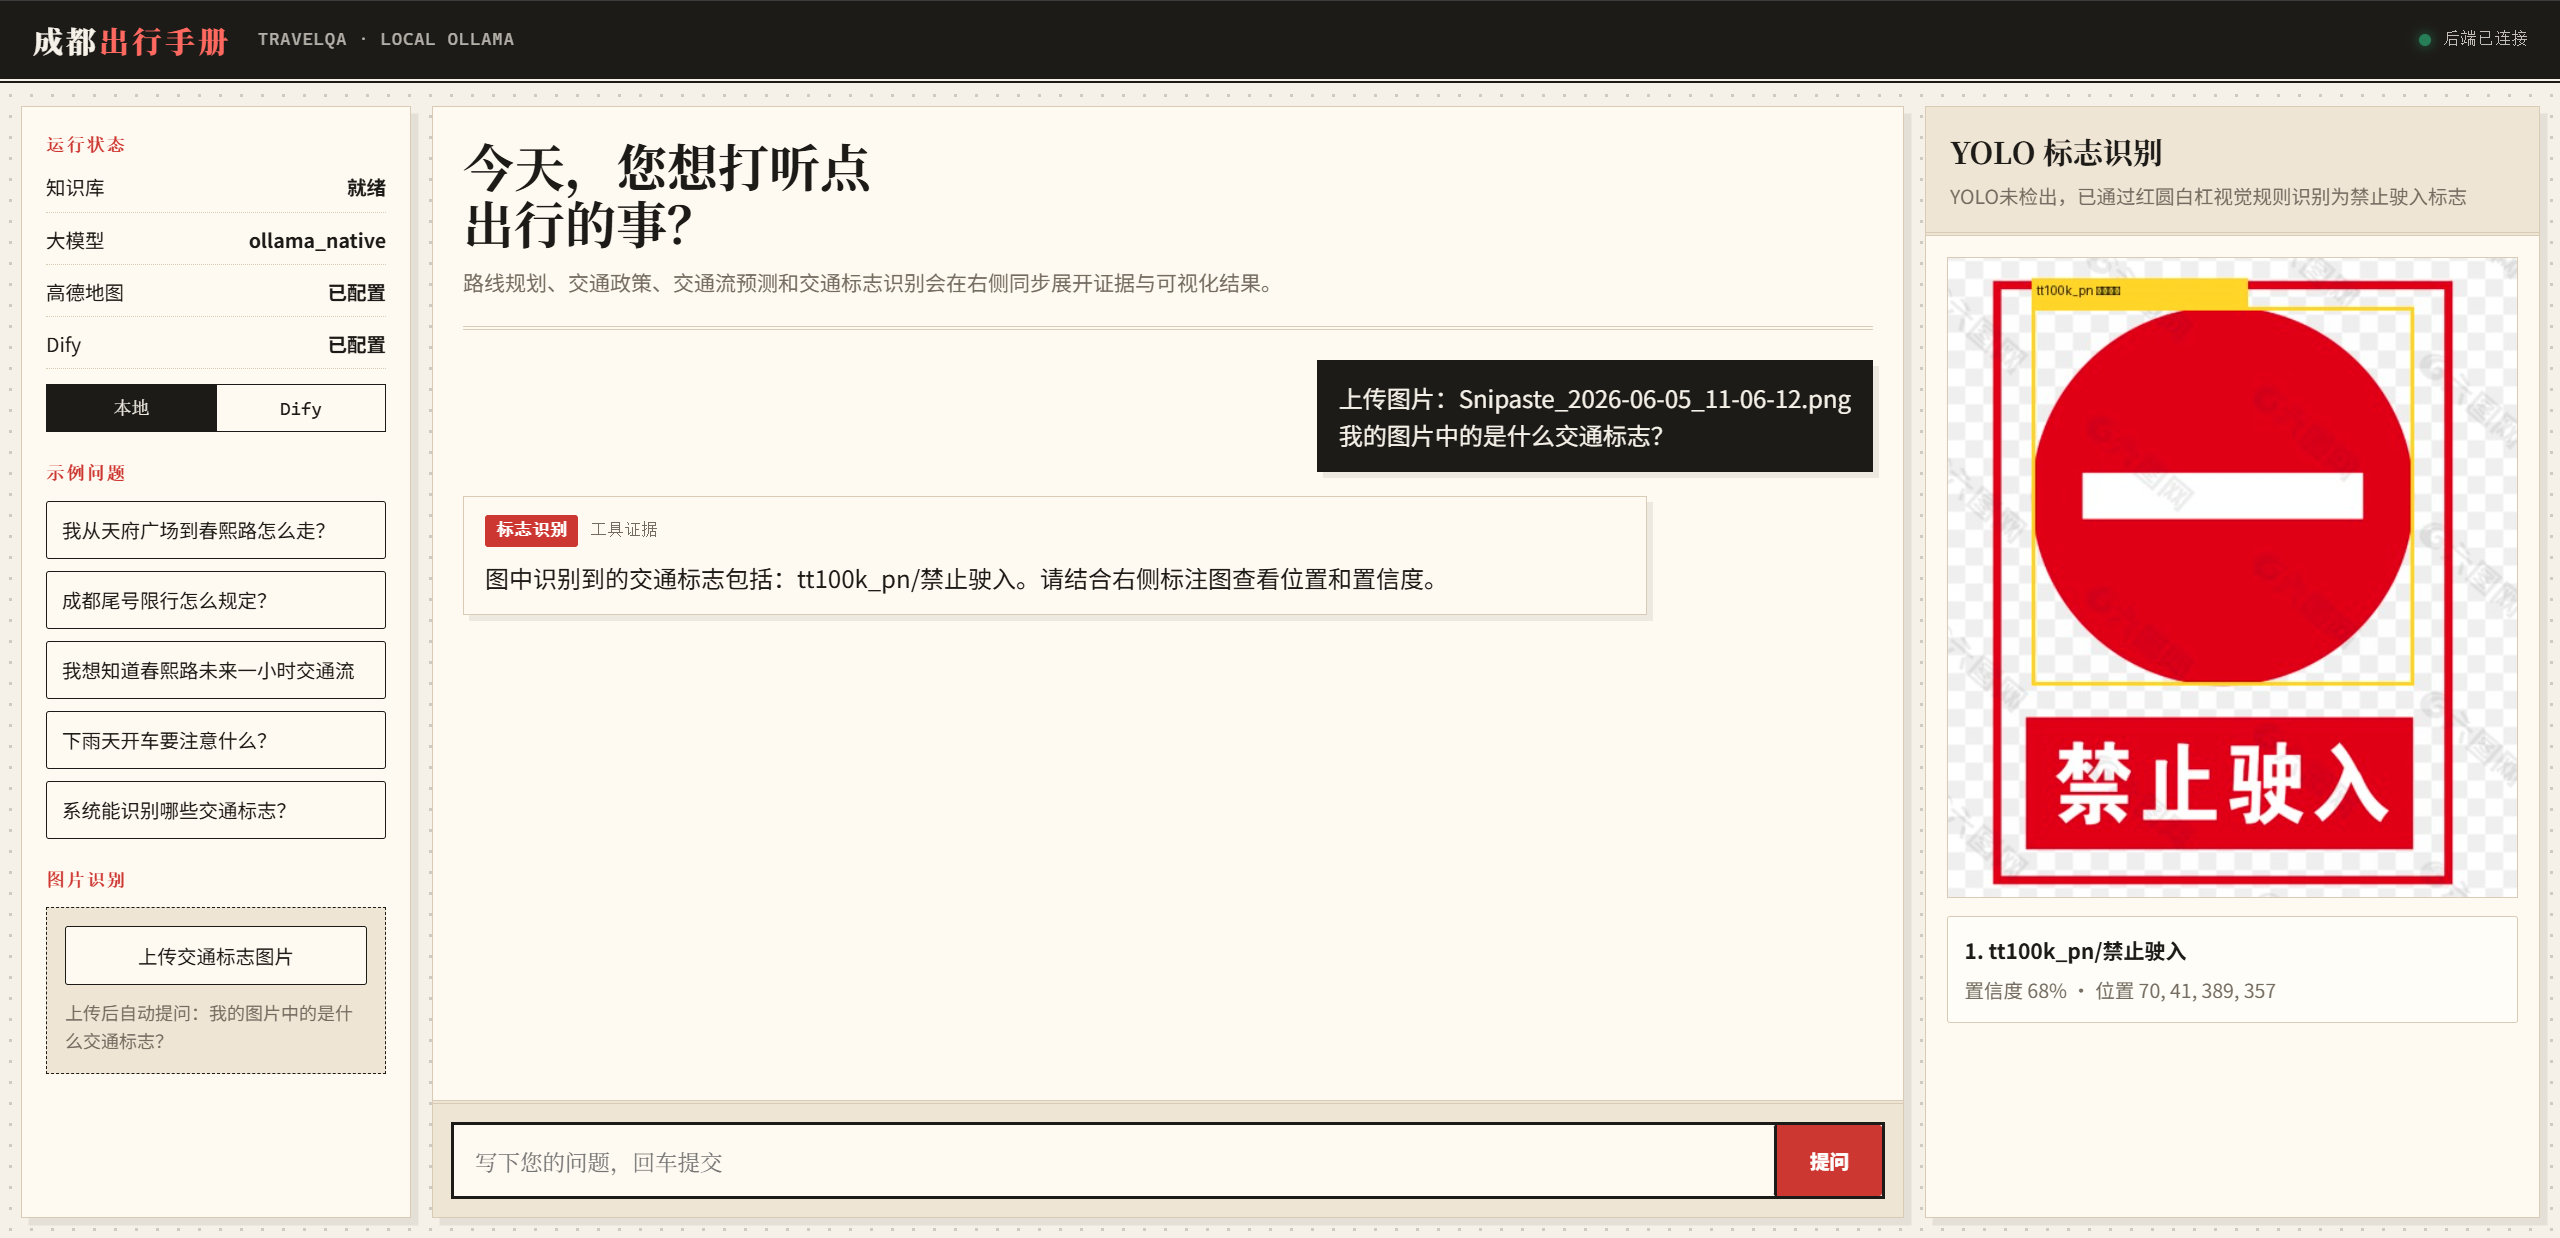
\includegraphics[width=0.96\textwidth]{figures/ui_detection_result.png}
    \caption{交通标志识别问答界面}
    \label{fig:ui-detection-result}
\end{figure}

图\ref{fig:dify-logs} 展示了 Dify 工作流的运行日志。日志中可以看到路线规划、交通流预测、限行问答等多类请求均由 \texttt{travelqa-web} 用户触发，并获得成功状态，说明前端、后端代理和 Dify 工作流之间的调用链路已经打通。

\begin{figure}[H]
    \centering
    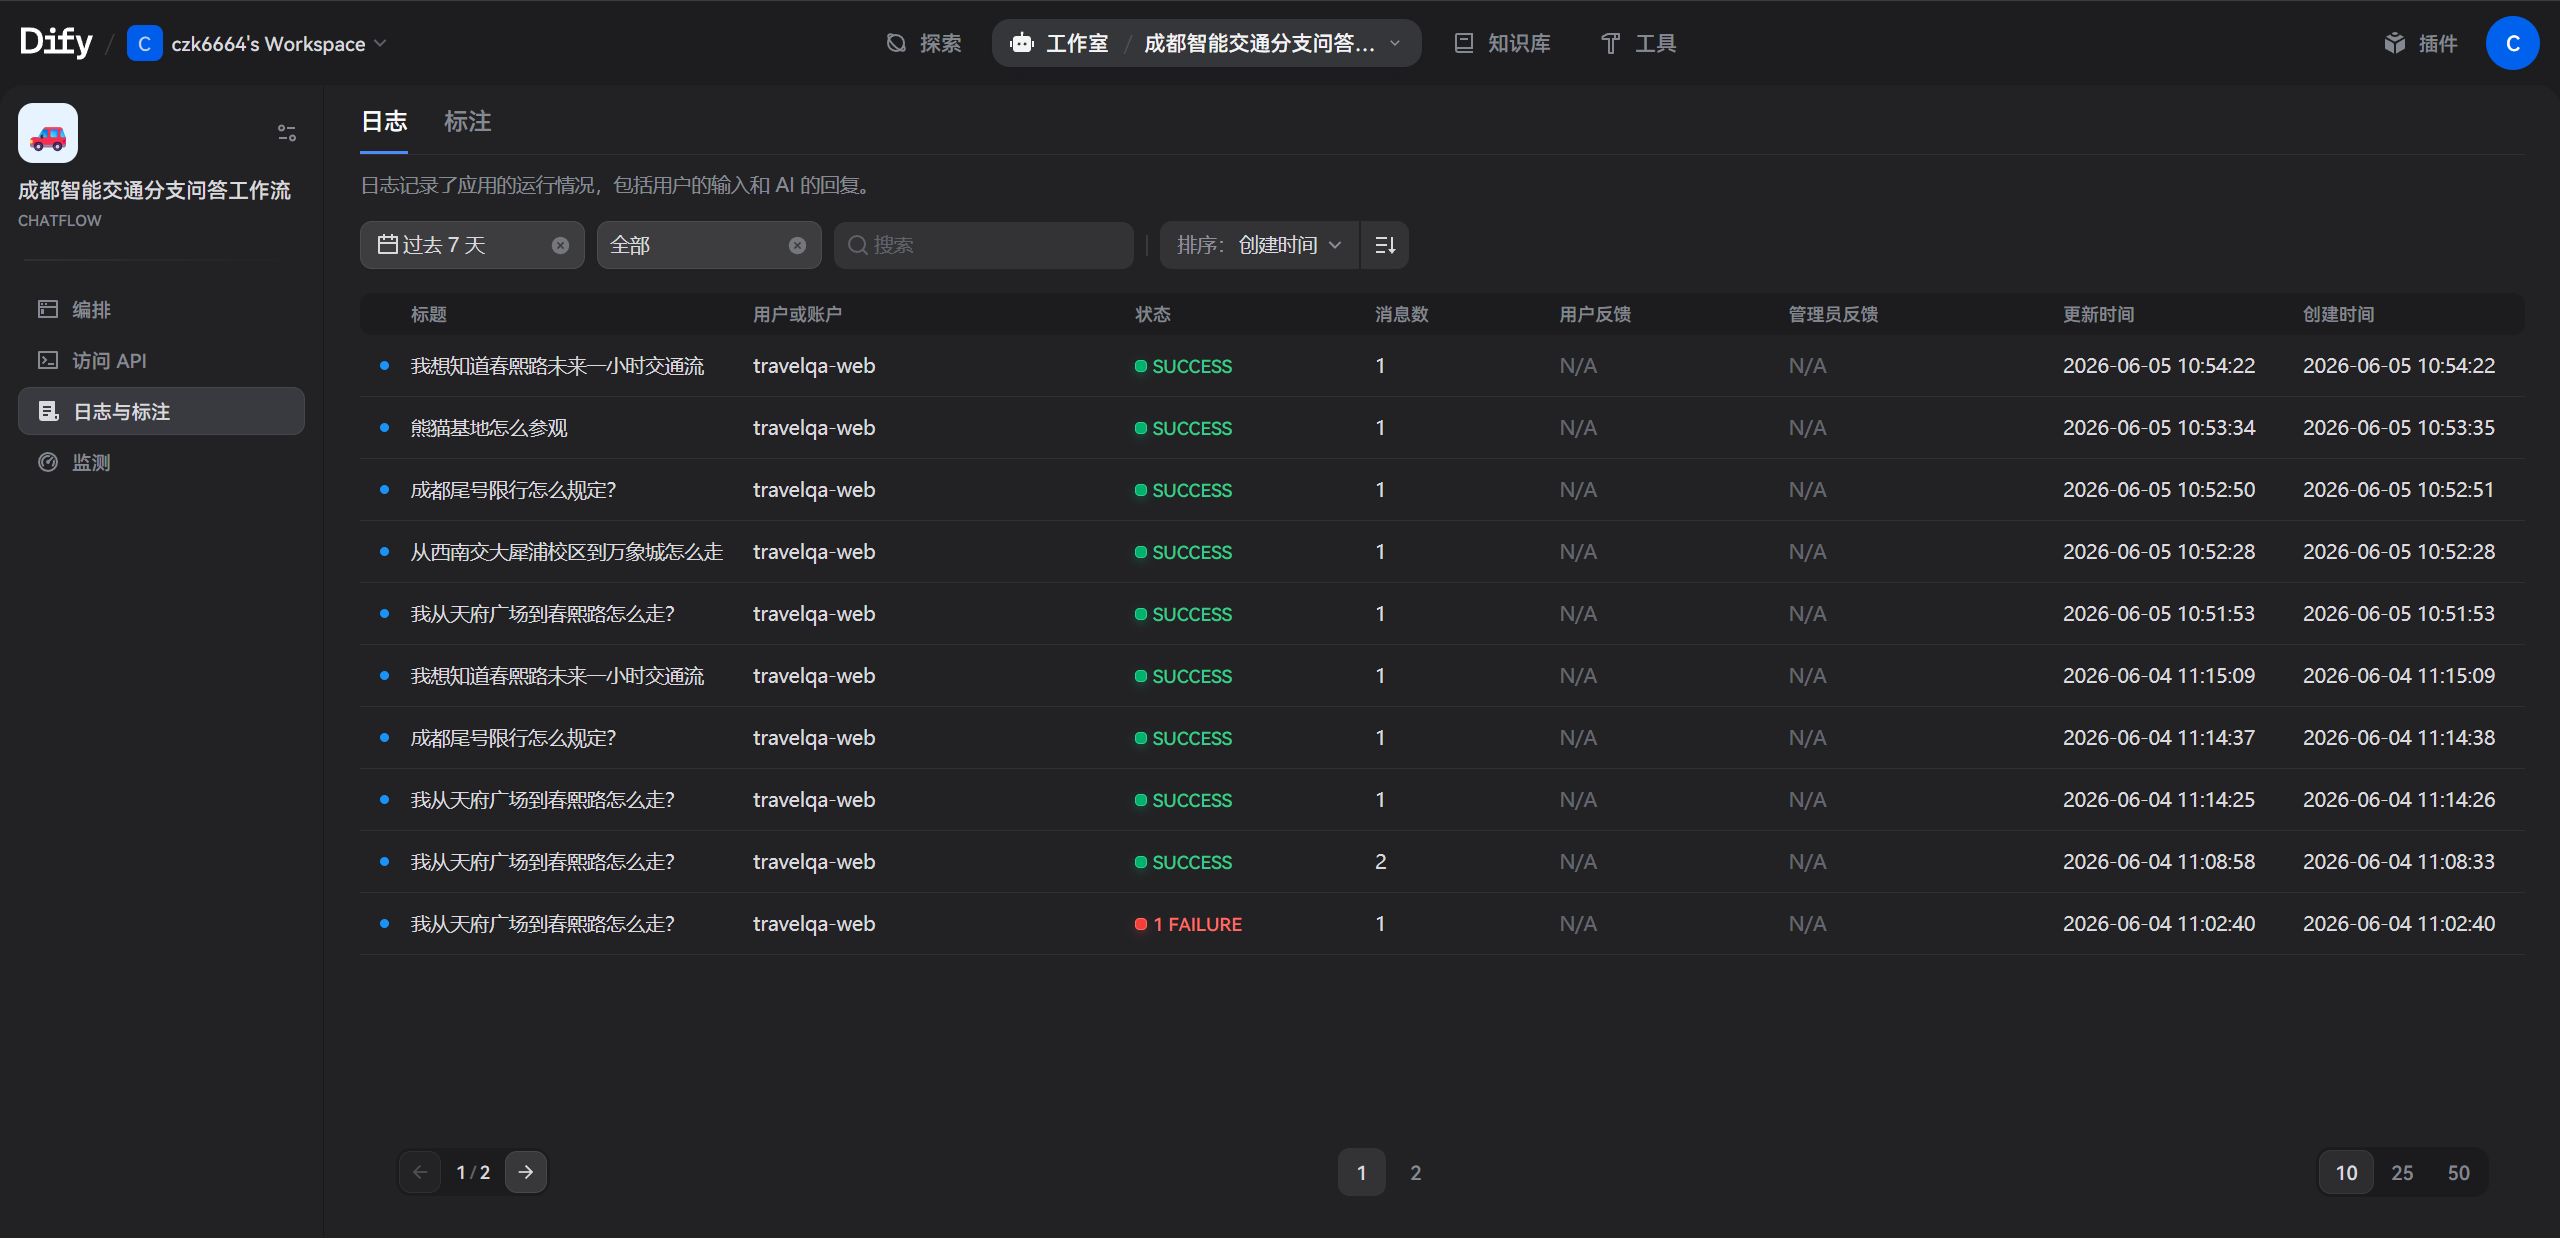
\includegraphics[width=0.96\textwidth]{figures/dify_logs.png}
    \caption{Dify 工作流日志页面}
    \label{fig:dify-logs}
\end{figure}

图\ref{fig:dify-monitor} 展示了 Dify 监控页面。监控面板记录会话数量、活跃用户、平均互动数和 Token 输出速度等指标，可用于观察演示和测试过程中的运行状态。

\begin{figure}[H]
    \centering
    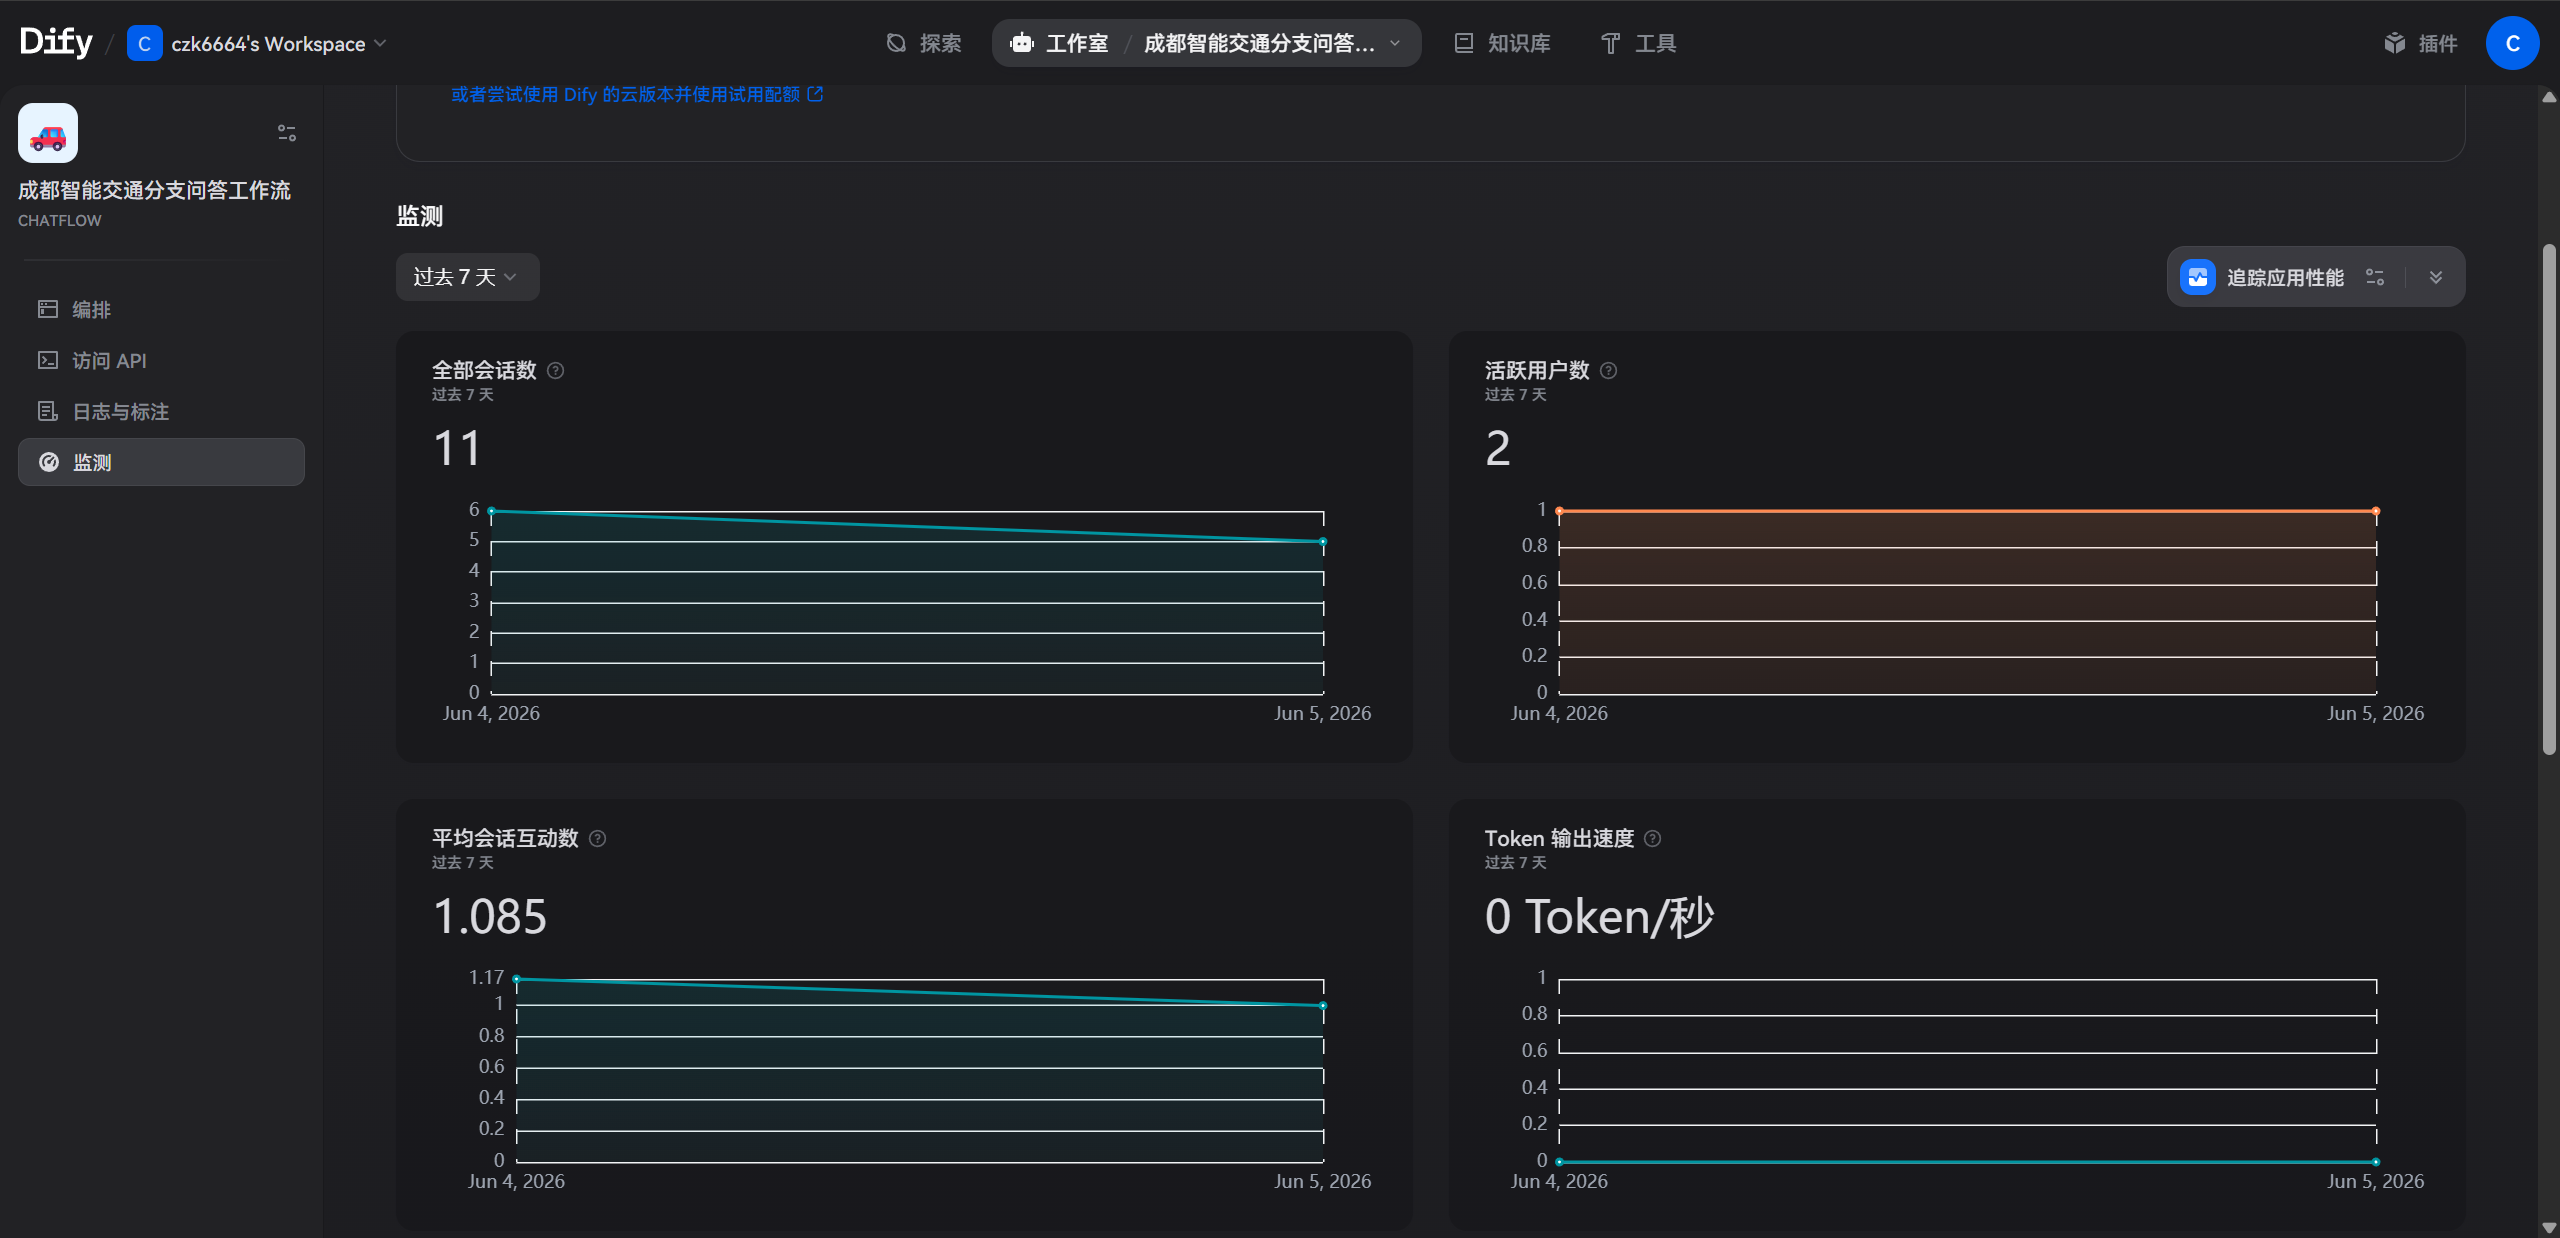
\includegraphics[width=0.96\textwidth]{figures/dify_monitor.png}
    \caption{Dify 工作流监控页面}
    \label{fig:dify-monitor}
\end{figure}

\subsection{错误处理验证}
错误处理测试不是为了说明系统已经很完善，而是为了防止演示时出现空白页面。现场环境可能和开发环境不一样，例如地图 Key 没配、Dify 未发布、Docker 没启动或 YOLO 权重缺失。遇到这些情况时，系统至少要返回可读提示，让用户知道为什么没有完整结果，而不是让模型继续编或让页面直接崩溃：
\begin{itemize}
    \item 高德 JS Key 缺失：前端地图降级为路线摘要和 polyline 简图。
    \item 高德 Web 服务失败：后端返回 \texttt{available=false} 和错误原因。
    \item YOLO 模型缺失：返回模型不可用提示。
    \item Dify 未发布：后端返回 Dify 调用失败，提示 \texttt{Workflow not published}。
    \item Docker 未启动：一键启动脚本尝试启动 Docker Desktop 并等待就绪。
\end{itemize}

这部分对课程演示比较重要。比如地图配置缺失时，系统至少还能给出路线摘要；Dify 调用失败时，本地模式仍然可以用于展示主要功能。后续还需要把知识库无命中、外部搜索结果过旧、图片未上传等情况的提示写得更细。

\section{结果分析}
这次项目真正跑通的是一条综合问答流程，而不是单独的聊天页面。Dify 工作流、DeepSeek 基座模型与 LoRA/QLoRA 微调、本地 RAG 知识库、高德路线规划、天气查询、知乎补充、STAEformer 预测和 YOLO 识别都在系统中有对应入口。用户提问后，页面不只显示一段回答，还能在右侧看到地图、知识片段、预测曲线或识别标注图。

实际开发时可以发现，问答系统的难点不只是让模型说话。更麻烦的是回答、证据和工具结果要对得上。RAG 对交通问答很重要，因为政策和公告不能只靠模型记忆；高德和天气工具能减少实时信息编造；三栏界面对调试很有帮助，因为可以同时看到回答和依据。FastAPI 在这里起到了统一封装的作用，本地 Web 前端和 Dify 工作流都调用同一套后端接口。Dify 模式下，后端代理负责调用工作流，本地后端再补建 panel，因此工作流回答和本地可视化结果可以放在同一个页面里。

交通流预测部分需要单独说明。当前使用的是成都地点到 PEMS08 节点的演示映射，所以它证明的是``大作业1预测模型可以作为工具节点被问答系统调用并可视化''，不能说明系统已经具备真实成都道路预测能力。报告和前端都标注了这个限制。以后如果能接入成都真实检测器或交通指数数据，现有 \texttt{ForecastTool}、Dify 节点和右侧折线图 panel 仍然可以继续复用。

评测材料主要用于说明链路确实跑过，而不是把系统包装成成熟产品。RAG 知识库规模、LoRA 数据规模、离线功能评测、扩展意图评测、RAG Top-K 来源命中率、RAG 消融结果、RAG 压力集、端到端延迟、A/B 规则化评分和 20 条人工盲评都可以在项目目录中复查。这里也要承认，RAG Top-K 评测验证的是来源召回，不等于最终回答已经完成全自动事实核验；A/B 评分主要看工具调用意识、拒答边界和思维泄漏控制；人工盲评样本数量也还不大。

\section{不足与改进方向}
目前系统还不能当成真实交通服务使用，主要问题集中在数据、实时性、模型边界和部署环境上：
\begin{enumerate}
    \item 本地知识库目前仍是有限文档和有限 chunk，临时交通公告、短期施工信息和具体路段覆盖还不够，政策类问题仍需要定期更新。
    \item 交通流预测尚未接入真实成都传感器数据，当前为成都地点名到 PEMS08 节点的演示映射，因此不能把预测值解释为真实成都路段流量。
    \item \texttt{DeepSeek-R1-Distill-Qwen-7B} 模型卡参数量为 7.62B，属于 7B 级蒸馏模型；若评分严格限定 1--7B 字面范围，应准备 1.5B 或 \texttt{deepseek-llm-7b-chat} 替代方案。
    \item RAG 已完成 20 条来源 Top-K、12 条压力集和小规模消融，但压力集显示 4 条负例中仍有 2 条近似成都时效问题会召回相近公告，需要增加实体一致性和发布时间检查。
    \item LoRA 微调数据量不算大，而且更偏向回答边界和工具意识，不代表模型真正掌握了完整交通知识。当前 100 条 A/B 规则化评分和 20 条人工盲评只能作为小规模复核。
    \item 知乎搜索结果质量不稳定，只能作为经验性参考，不能作为政策依据。后续需要继续加入时间、来源可信度和内容相关性过滤。
    \item 规则意图识别稳定、容易调试，但灵活性不足。遇到混合问题或问法变化较大的问题时，仍可能需要 LLM 分类或更细的规则补充。
    \item 图片识别依赖本地 YOLO 权重和运行环境，只覆盖已训练类别，不能识别所有交通标志。首次部署时还要检查模型文件和依赖是否完整。
    \item 前端采用原生 HTML/CSS/JavaScript，适合课程演示，但后续如果加入复杂多轮交互，维护成本会提高。
    \item Dify 模式依赖本地后端、容器网络和密钥配置，换环境时仍需要重新检查；Dify 原生知识库能力目前也没有深入配置。
    \item 前端地图展示依赖高德 JS API Key，未配置时只能使用降级展示，路线可视化效果会受影响。
\end{enumerate}

后续如果继续做，优先可以从以下方向推进：
\begin{itemize}
    \item 优先补官方数据源和自动更新机制，而不是单纯继续堆提示词。
    \item 如果继续做交通流预测，应接入成都市真实道路传感器或开放交通指数数据，逐步替换当前演示映射。
    \item 在 Dify LLM 分类节点中复用 \texttt{run\_intent\_compare.py} 的 few-shot prompt，补充规则分类与 LLM 分类的在线对比结果，并保留规则路由作为离线降级路径。
    \item 扩展 RAG 压力集并增加实体一致性校验、发布时间校验和低分拒答阈值，补充最终回答准确率、引用正确率和人工事实核验。
    \item 在现有 \texttt{score\_ab\_eval.py} 与 \texttt{ab\_blind\_review\_20.json} 基础上扩大人工评分样本，继续报告微调前后在流畅度、完整性和引用表达质量上的差异。
    \item 在 Dify 中进一步配置原生知识库、模型供应商和工具插件，同时保留后端代理来管理密钥和工具调用。
    \item 前端可以逐步增加用户会话记忆和多轮路线澄清能力，但需要避免把页面逻辑写得过散。
    \item YOLO 部分可以先扩展更多交通标志类别，再考虑视频流实时检测。
\end{itemize}

\section{总结}
这次课程设计最后完成的是一个能演示的智能交通问答原型。它把 Dify 工作流、本地 RAG、高德地图 API、天气查询、知乎搜索补充、STAEformer 交通流预测和 YOLO 交通目标识别放到了同一个页面里。相比单独做一个聊天机器人，这个项目更强调回答背后的依据和工具结果。

实现过程中，我们以 FastAPI 后端统一封装各类接口，使用 \texttt{DeepSeek-R1-Distill-Qwen-7B} 作为基座并完成 LoRA/QLoRA 微调；知识库采集成都市交管局信息发布栏，并结合交通法规资料构建本地 RAG。测试中，普通问答、RAG 证据、路线规划、天气提醒、预测曲线、图片识别和 Dify 工作流调用都能跑通。真正做下来后可以看到，模型适合整理语言，但路线、天气、政策依据和图片识别都需要外部结果支撑。

当前版本已经覆盖课程要求中的主要模块，但它仍然是课程设计原型。知识库规模有限，交通流预测还是演示映射，部分意图识别依赖规则，外部 API 也受网络和密钥影响。这次项目的实际收获是把模型回答、工具调用和证据展示放到了一条链路里，也看到了其中的边界问题。后续如果继续完善，优先应该补充官方数据源和真实交通数据，扩大评测样本，并把 RAG 边界判断和前端交互做得更稳。

\begin{thebibliography}{99}
\bibitem{rag} Lewis P, Perez E, Piktus A, et al. Retrieval-Augmented Generation for Knowledge-Intensive NLP Tasks. NeurIPS, 2020.
\bibitem{deepseekr1} DeepSeek-AI. DeepSeek-R1: Incentivizing Reasoning Capability in LLMs via Reinforcement Learning. arXiv:2501.12948, 2025.
\bibitem{modelscope} ModelScope. DeepSeek-R1-Distill-Qwen-7B 模型介绍. \url{https://modelscope.cn/models/deepseek-ai/DeepSeek-R1-Distill-Qwen-7B}
\bibitem{bm25} Robertson S, Zaragoza H. The Probabilistic Relevance Framework: BM25 and Beyond. Foundations and Trends in Information Retrieval, 2009.
\bibitem{dify} Dify Documentation. Dify Workflow and Chatflow Documentation. \url{https://docs.dify.ai/}
\bibitem{amap} 高德开放平台. 高德 Web 服务 API 与 JavaScript API 文档. \url{https://lbs.amap.com/}
\bibitem{staeformer} Liu H, et al. Spatio-Temporal Adaptive Embedding Makes Vanilla Transformer SOTA for Traffic Forecasting. CIKM, 2023.
\bibitem{yolo} Jocher G, Chaurasia A, Qiu J. Ultralytics YOLO. \url{https://github.com/ultralytics/ultralytics}
\bibitem{tt100k} Zhu Z, Liang D, Zhang S, et al. Traffic-Sign Detection and Classification in the Wild. CVPR, 2016.
\bibitem{zhihuapi} 知乎开放平台. 知乎搜索 API 文档.
\end{thebibliography}

\end{document}

